%%%%%%%%%%%%%%%%%%%%%%%%%%%%%%%%%%%%%%%%%%%%%%%%%%%%%%%%%%%%%%%%%%%%%%%%%%%%%%%%
%2345678901234567890123456789012345678901234567890123456789012345678901234567890
%        1         2         3         4         5         6         7         8

%\documentclass[journal,transmag]{IEEEtran}% Comment this line out if you need a4paper

\documentclass[10pt, conference]{ieeeconf}      % Use this line for a4 paper

\IEEEoverridecommandlockouts                              % This command is only needed if 
                                                          % you want to use the \thanks command

%\overrideIEEEmargins                                      % Needed to meet printer requirements.

% See the \addtolength command later in the file to balance the column lengths
% on the last page of the document

% The following packages can be found on http:\\www.ctan.org
%\usepackage{graphics} % for pdf, bitmapped graphics files
%\usepackage{epsfig} % for postscript graphics files
%\usepackage{mathptmx} % assumes new font selection scheme installed
%\usepackage{times} % assumes new font selection scheme installed
%\usepackage{amsmath} % assumes amsmath package installed
%\usepackage{amssymb}  % assumes amsmath package installed



\usepackage{amsmath,amssymb}

\usepackage{tikz,hyperref,graphicx,units,subfig}
\usepackage{subfig}
\usepackage{benktools}
\usepackage{caption}
\usepackage{epstopdf}
\renewcommand{\captionfont}{\footnotesize}
\usepackage{sidecap,wrapfig}
\usepackage[ruled,vlined]{algorithm2e}
\DeclareMathOperator*{\argmin}{arg\,min}
\DeclareMathOperator*{\argmax}{arg\,max}
\newcommand{\abs}[1]{\lvert#1\rvert} 
\newcommand{\norm}[1]{\lVert#1\rVert}
%\newcommand{\suchthat}{\mid}
\newcommand{\suchthat}{\ \big|\ }
\newcommand{\ba}{\mathbf{a}}
\newcommand{\bb}{\mathbf{b}}
\newcommand{\bc}{\mathbf{c}}
\newcommand{\bd}{\mathbf{d}}
\newcommand{\bg}{\mathbf{g}}
\newcommand{\bj}{\mathbf{j}}
\newcommand{\bn}{\mathbf{n}}
\newcommand{\bp}{\mathbf{p}}
\newcommand{\bw}{\mathbf{w}}
\newcommand{\bt}{\mathbf{t}}
\newcommand{\by}{\mathbf{y}}
\newcommand{\bx}{\mathbf{x}}
\newcommand{\bz}{\mathbf{z}}
\newcommand{\bbf}{\mathbf{f}}
\newcommand{\bzero}{\mathbf{0}}
\newcommand{\bG}{\mathbf{G}}
\newcommand{\bA}{\mathbf{A}}
\newcommand{\bW}{\mathbf{W}}
\newcommand{\bX}{\mathbf{X}}
\newcommand{\mX}{\mathcal{X}}
\newcommand{\mD}{\mathcal{D}}
\newcommand{\mG}{\mathcal{G}}
\newcommand{\mN}{\mathcal{N}}
\newcommand{\mW}{\mathcal{W}}
\newcommand{\mF}{\mathcal{F}}
\newcommand{\bZ}{\mathbf{Z}}

\newcommand{\bfc}{W}
\newcommand{\Qinf}{Q_{\infty}}
\newcommand{\st}[1]{_\text{#1}}
\newcommand{\rres}{r\st{res}}
\newcommand{\pos}[1]{(#1)^+}
\newcommand{\depth}{\operatorname{depth}}
\newcommand{\dist}{\operatorname{dist}}
\newcommand{\convhull}{\operatorname{ConvexHull}}
\newcommand{\minksum}{\operatorname{MinkowskiSum}}

\title{\LARGE \bf
Multi-Arm Bandit Models for 2D Grasp Planning with Uncertainty  [v7 Feb 18, 2015 ] }


\author{Michael Laskey$^1$, Jeff Mahler$^1$, Zoe McCarthy$^1$,  Florian T. Pokorny$^3$, Sachin Patil$^1$,\\ Jur Van Den Berg$^4$,  Danica Kragic$^3$, Pieter Abbeel$^1$, Ken Goldberg$^2$% <-this % stops a space
\thanks{$^1$Department of Electrical Engineering and Computer Sciences; {\small \{mdlaskey, zmccarthy, jmahler, sachinpatil, pabbeel\}@berkeley.edu}}%
\thanks{$^2$Department of Industrial Engineering and Operations Research and Department of Electrical Engineering and Computer Sciences; {\small goldberg@berkeley.edu}}%
\thanks{$^{1-2}$ University of California, Berkeley;  Berkeley, CA 94720, USA}%
\thanks{$^3$Computer Vision and Active Perception Lab, Centre for Autonomous Systems, School of Computer Science and Communication, KTH Royal Institute of Technology, Stockholm, Sweden {\small \{fpokorny, dani\}@kth.se}}%
\thanks{$^4$Google; Amphitheatre Parkway, Mountain View, CA 94043, USA {\small jurvandenberg@gmail.com}}%
} 

\newtheorem{theorem}{Theorem}

\begin{document}



\maketitle
\thispagestyle{empty}
\pagestyle{empty}


%%%%%%%%%%%%%%%%%%%%%%%%%%%%%%%%%%%%%%%%%%%%%%%%%%%%%%%%%%%%%%%%%%%%%%%%%%%%%%%%

\begin{abstract}
Sampling perturbations in shape, state, and control can facilitate grasp planning in the presence of uncertainty arising from noise, occlusions, and surface properties such as transparency and specularities. 
Monte-Carlo sampling is a popular approach to grasp planning under uncertainty, but it may require a large number of samples to converge, even for planar models.
We consider an alternative based on the multi-armed bandit (MAB) model for making sequential decisions.
We formulate grasp planning as a MAB  to efficiently determine high quality grasp with respect to a probability of force closure metric.
We compare against two previously proposed methods for grasp selection uniform allocation, or uniformly selecting samples, and an adaptive sampling approach known as Iterative Pruning, which iteratively reduces the set of candidate grasps. We consider the case of shape uncertainty represented as a Gaussian process implicit surface (GPIS) and Gaussian uncertainty in pose, grasp approach direction, and coefficient of friction.
In simulation, initial results  showed that given 1000 randomly selected grasps the number of samples required, on average over 100 objects, to get within $2.5\%$ of the estimated highest probability of force closure an MAB algorithm used $439\%$ fewer samples than the sample mean based adaptive sampling approach previously used.
\end{abstract}


%%%%%%%%%%%%%%%%%%%%%%%%%%%%%%%%%%%%%%%%%%%%%%%%%%%%%%%%%%%%%%%%%%%%%%%%%%%%%%%%

\section{Introduction}


%\vspace{10pt}
%\todo{Get High res GPIS visualizations, Incorporate next round of feedback}

Consider a robot fulfilling orders in a warehouse, where it encounters new consumer products and must handle them quickly. Planning grasps using analytic methods, requires the contact locations and surface normals. The robot may not be able to measure these quantities exactly due to sensor imprecision and missing data, which could result from occlusions, transparency, or highly reflective surfaces. 

% \begin{figure}%
%     \centering
% %     \subfloat{{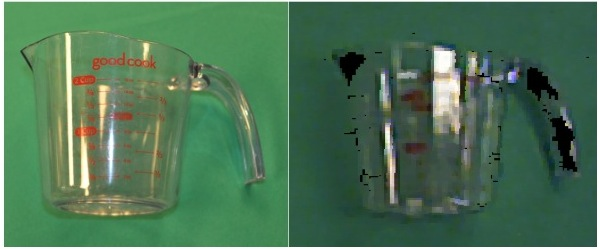
\includegraphics[width=8cm]{figures/cup.jpg} }}%
% %       \qquad
  
%      \subfloat{{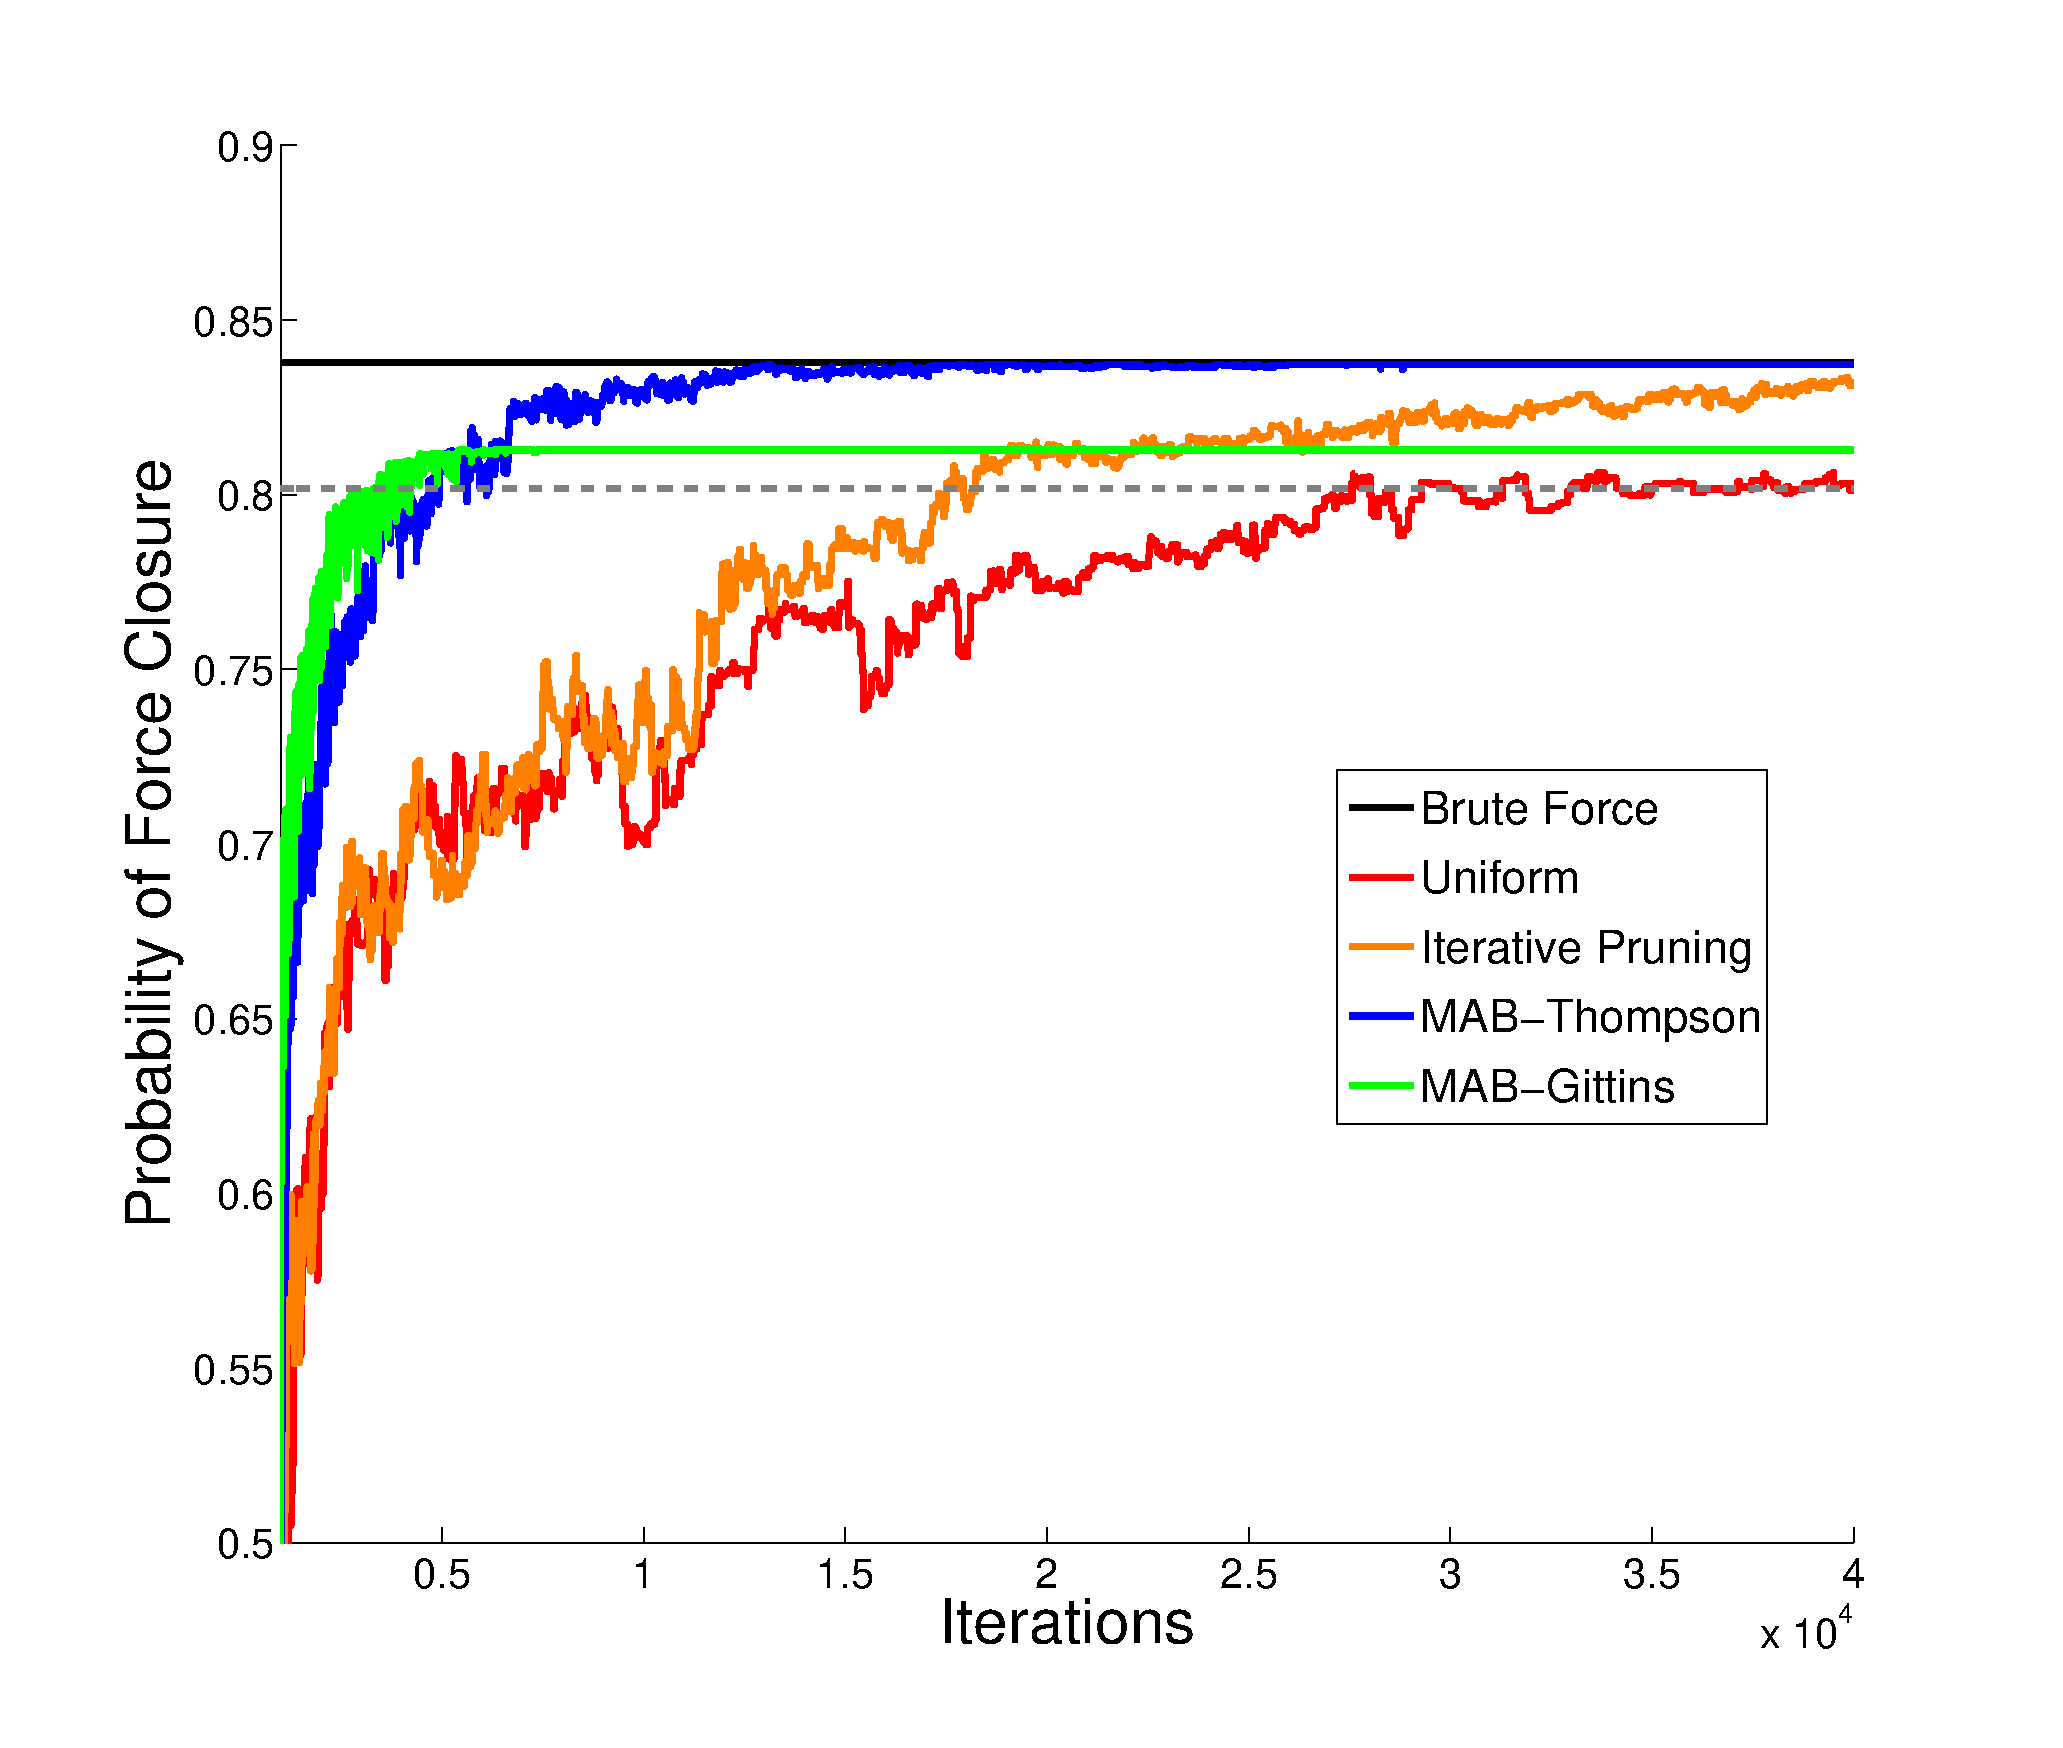
\includegraphics[width=8.5cm]{matlab_figures/pfc.eps} }}%
   
%     \caption{ Comparison of the current average probability of force closure vs. the stopping time $T_s$. The plots are averaged over 100 shapes randomly drawn from the Brown Vision 2D Lab Dataset \cite{brown} with $|G|=1000$ for each shape.  We demonstrate this for Thompson, Gittins, Monte-Carlo and the approach of Kehoe et al \cite{kehoe2012toward}. We also plot the average probability of force closure for the estimated optimal grasp evaluated using Monte-Carlo sampling. Empirically, it appears that Thompson and Gittins converge to the optimal solution at a faster rate, which is desired for an anytime algorithm.   }%
%     \label{fig:rot_shapes}%
% \end{figure}

\begin{figure}%
    \centering
     \subfloat{{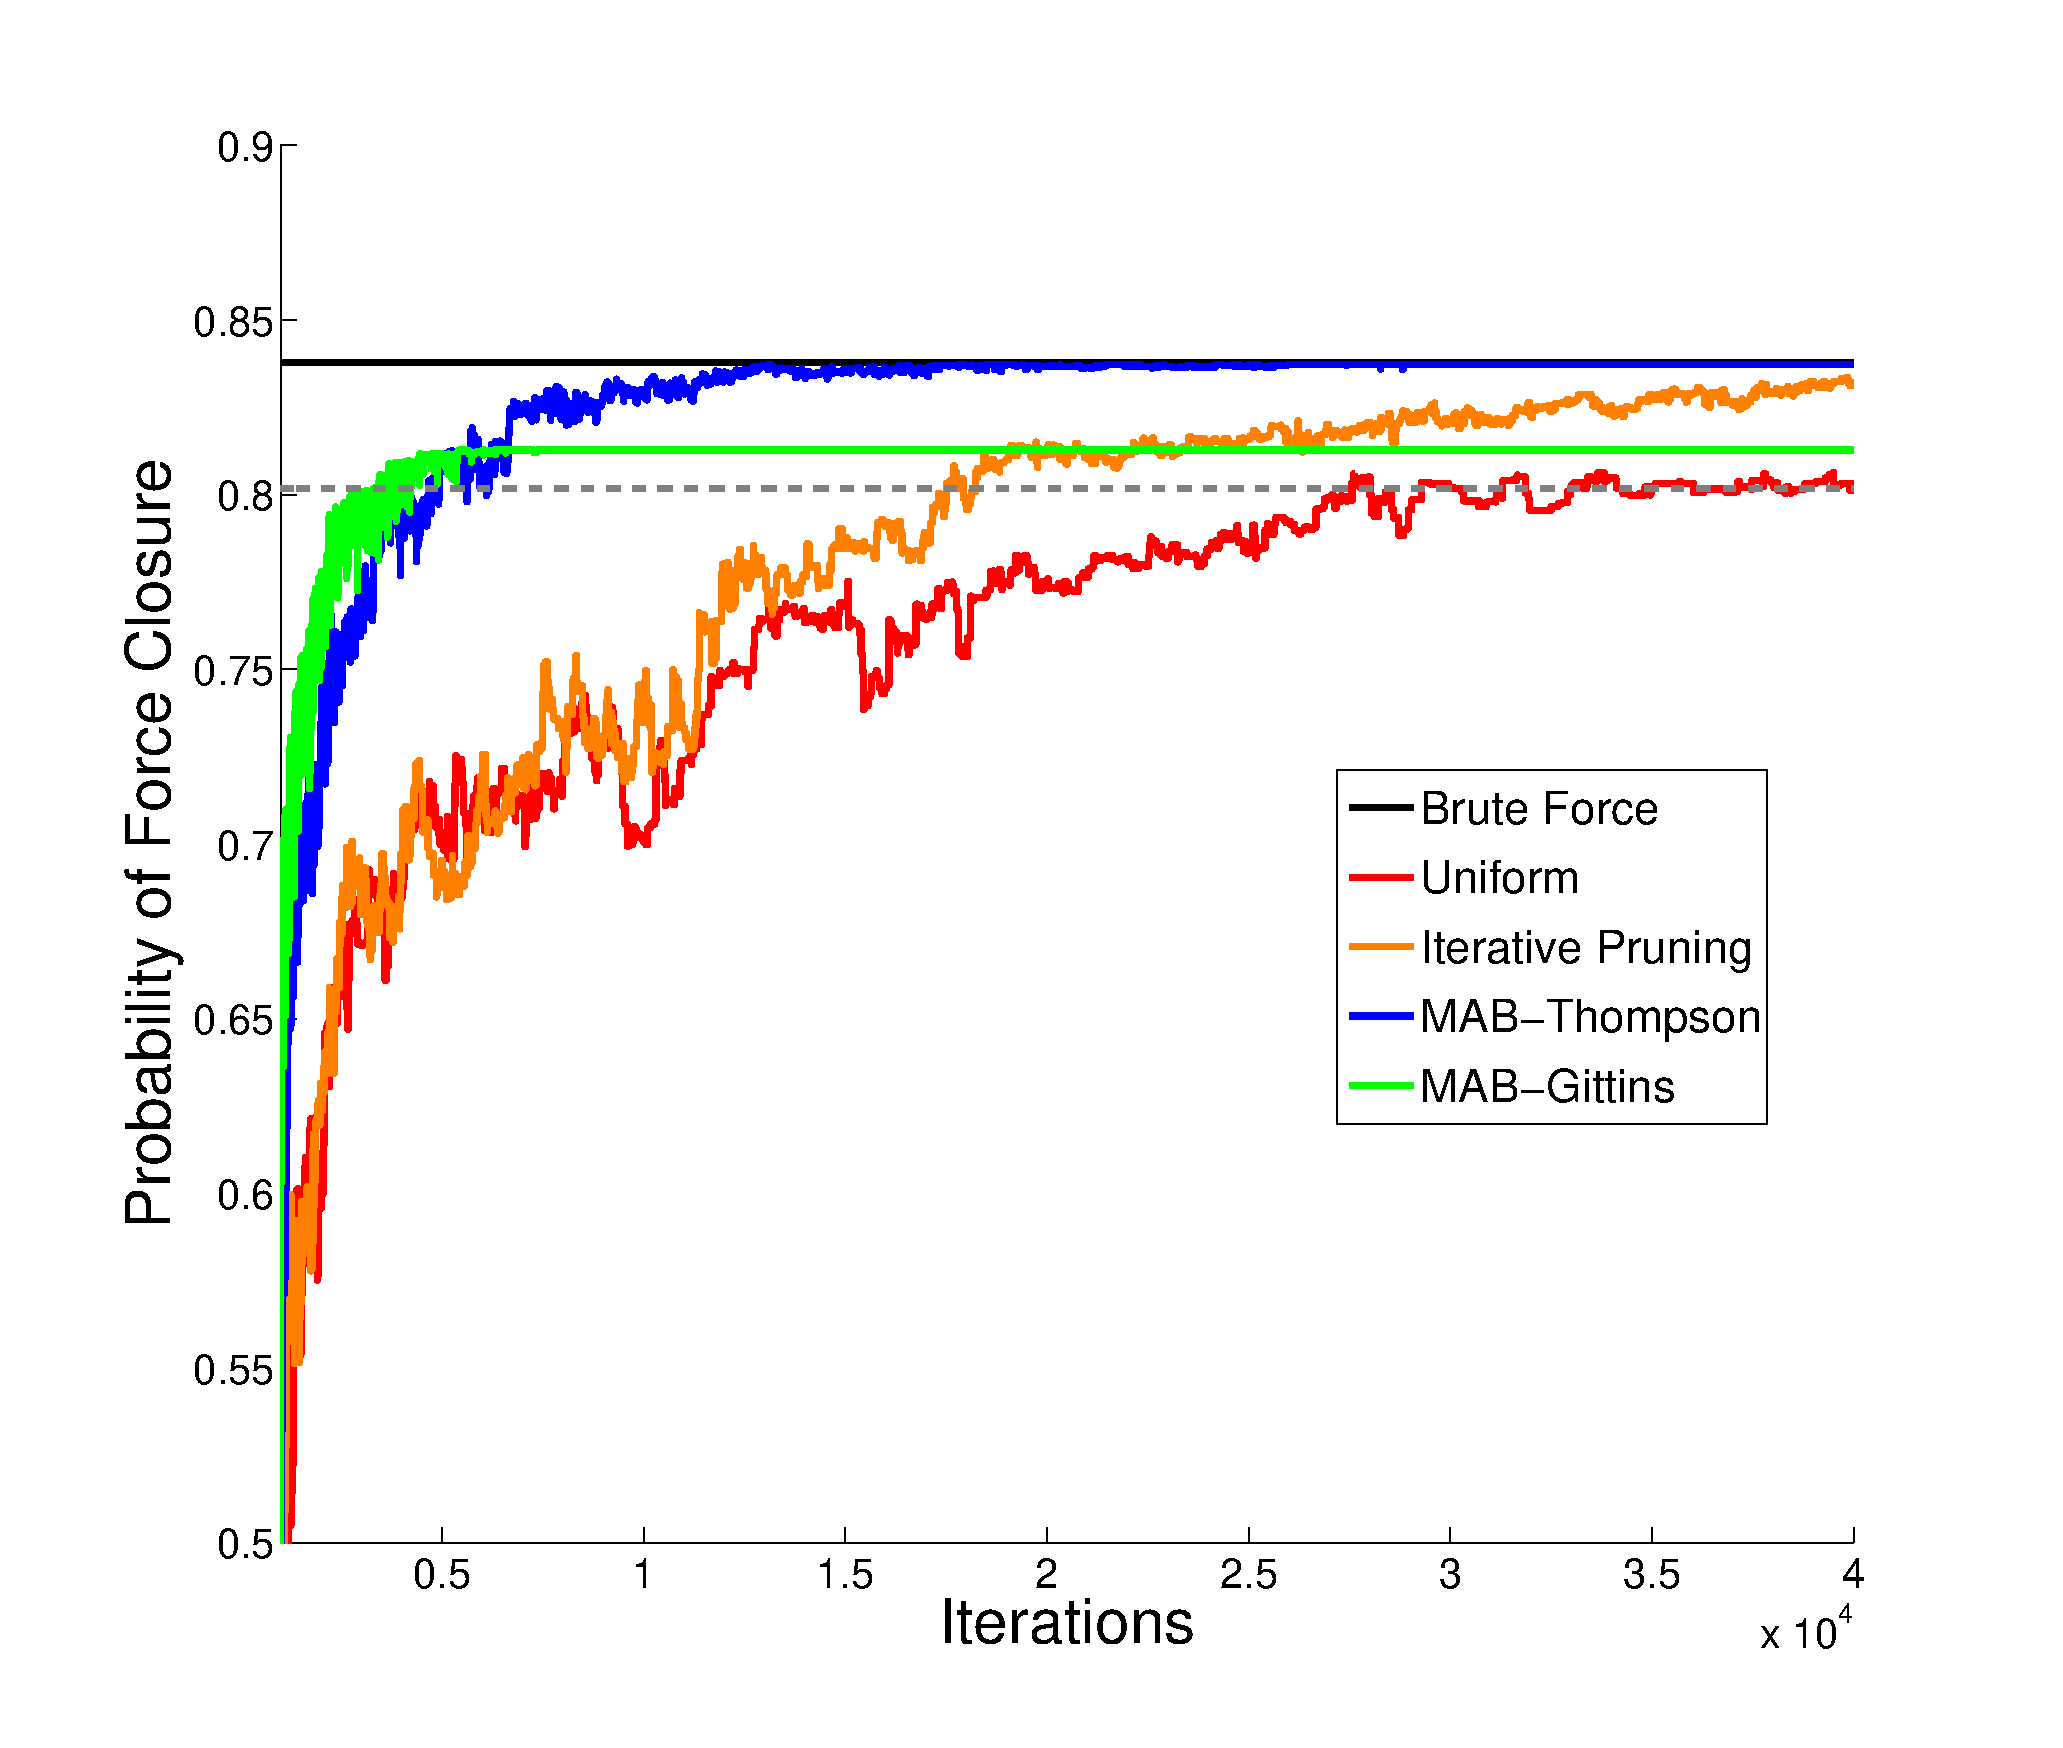
\includegraphics[scale=0.25]{matlab_figures/pfc.eps} }}%

    \caption{Comparison of the current average probability of force closure vs. the stopping time $T_s$.Graph is averaged over 100 shapes randomly drawn from the Brown Vision 2D Lab Dataset \cite{brown} with a set $|G|=1000$ for each shape.  We demonstrate this for Thompson, Gittins, uniform allocation and Iterative Pruning \cite{kehoe2012estimating}. We also demonstrate what the average highest probability of force closure is when the brute force approach of exhaustively sampling each candidate grasp is used. Empirically, it appears that Thompson and Gittins converge at a faster rate to the optimal solution, which is desired for an anytime algorithm  }%
    \label{fig:grasp_quality}
\end{figure}


One common measure of quality is force closure, the ability to resist external forces and torques in arbitrary directions~\cite{li1988task}.
Grasps in force closure can be further ranked by the relative magnitude of forces and torques that must be exerted by the gripper to resist external perturbations~\cite{ferrari1992}.
Recent work has explored computing the probability of  force closure given uncertainty in pose~\cite{christopoulos2007handling, kim2012physically, weisz2012pose} and object shape~\cite{kehoe2012estimating, mahler2015gp}.
One option is using Monte-Carlo integration over the possible values of uncertain quantities to evaluate the probability of force closure for a grasp~\cite{christopoulos2007handling, kim2012physically, weisz2012pose, kehoe2012estimating, kehoe2012toward}, but this can be computationally expensive due to the need to exhaustively sample every grasp candidate. 
We show that by using a Multi-Armed Bandit model it is possible to rule out grasps with low probability of force closure and to allocate more sampling effort to grasps that are likely to be high quality.

The multi-armed bandit (MAB) model for sequential decision making~\cite{barto1998reinforcement, lai1985asymptotically, robbins1985some} provides a formal way to reason about allocating sampling effort. In a standard MAB there are a set of possible options, or `arms'~\cite{barto1998reinforcement}, that each return a numeric reward from a stationary distribution.The goal in a MAB problem is to  select a sequence of options to maximize expected reward. The MAB algorithm can be interpreted as an anytime algorithm, where at a provided stopping time the algorithm terminates and returns the estimated best grasp, with respect to a chosen metric, or continues running until a user defined confidence level is met. 

We formulate the problem of ranking a set of candidate grasps according to a quality metric in the presence of uncertainty as a MAB problem.
We study this formulation using probability of force closure~\cite{christopoulos2007handling, weisz2012pose, kehoe2012toward} as a quality metric under uncertainty in pose, shape, grasp approach direction, and friction coefficient. 
We model shape uncertainty using Gaussian process implicit surfaces (GPISs), a Bayesian representation of shape uncertainty that has been used in various robotic applications~\cite{dragiev2011, hollinger2013}. 
We model uncertainty in pose as a normal distributions around the orientation and translation of the object.
Uncertainty in motion is represented as a normal distribution around the end point of a planned gripper trajectory and uncertainty in friction coefficient is a normal distribution around an expected friction coefficient.

We compare the performance of Thompson sampling and Gittins indices, two popular algorithms for solving the MAB problem against uniform allocation, or randomely sampling grasps, and an adaptive sampling method known as Iterative Pruning, which reduces the set size based on sample mean, proposed by Kehoe et al. \cite{kehoe2012toward}. In the task of finding grasps with high probability of force closure on the Brown Vision 2D Dataset~\cite{brown, christopoulos2007handling}.
In simulation, initial results  showed that given 1000 randomly selected grasps the number of samples required, on average over 100 objects, to get within $2.5\%$ of the estimated highest probability of force closure an MAB algorithm used $439\%$ fewer samples than the sample mean adaptive sampling approach previously used .


\section{Related Work}

Most research on grasp planning focuses on finding grasps by maximizing grasp quality metric when object shape, object pose, and locations of contact with an object are precisely known~\cite{cheong2011output, ciocarlie2009}.
Grasp quality is often measured by the ability to resist external perturbations to the object in wrench space~\cite{ferrari1992, miller2004graspit}.
Past work on grasping under uncertainty has considered uncertainty in the state of a robtic gripper~\cite{goldberg1990bayesian, stulp2011learning}, uncertainty in contact locations with an object~\cite{zheng2005}.

Recent work has studied the effects of uncertainty in object pose and gripper positioning.
 Brook, Ciocarlie, and Hsiao~\cite{brook2011collaborative, hsiao2011bayesian} studied a Bayesian framework to evaluate the probability of grasp success given uncertainty in object identity, gripper positioning, and pose by simulating grasps on deterministic mesh and point cloud models.
Weisz et al.~\cite{weisz2012pose} found that grasps ranked by probability of force closure subject to uncertainty in object pose were empirically more successful on a physical robot grasps planned using deterministic wrench space metrics on objects from the Columbia Grasp Database.
Kim et al.~\cite{kim2012physically} planned grasps using dynamic simulations over perturbations in object pose, and also found that the planned grasps were more successful on a physical robot than classical grasp metrics.

Recent work has also studied uncertainty in object shape, motivated by the use of uncertain low-cost sensors and tolerances in part manufacturing.
Christopoulos et al.~\cite{christopoulos2007handling} sampled spline fits for 2-dimensional planar objects and ranked a set of randomly generated grasps by probability of force closure.
Kehoe et al.~\cite{kehoe2012estimating, kehoe2012toward} sampled perturbations in shape for extruded polygonal objects to plan push grasps for parallel-jaw grippers.
Several recent works have also studied using Gaussian process implicit surfaces (GPISs) to represent shape uncertainty due to its ability to represent arbitrary topologies and correlations between shape uncertainty over spatial locations~\cite{dragiev2011, dragiev2013uncertainty, hollinger2013, mahler2015gp}.
Dragiev et al.~\cite{dragiev2011} used the mean GPIS to control a grasp to reach a desired location, and extended this work to use GPIS for active tactile shape exploration during grasping~\cite{dragiev2013uncertainty}.
Mahler et al. used the GPIS representation to find locally optimal anti-podal grasps by framing grasp planning as an optimization problem~\cite{mahler2015gp}. 




Some probabilistic grasp quality measures, such as probability of force closure, use Monte-Carlo sampling to evaluate grasp quality~\cite{christopoulos2007handling, kehoe2012estimating, kehoe2012toward}.
This involves sampling from distributions on random quantities and averaging the quality over these samples to empirically estimate a probability distribution~\cite{caflisch1998monte}.
It can be computationally expensive though to sample all proposed grasps to convergence.
To address the computational cost, Kehoe et al.~\cite{kehoe2012estimating} proposed an adaptive sampling procedure known as Iterative Pruning, which at a set iteration discards a subset of the grasps that seem unlikely to be of high quality . However, the method pruned grasps using only the sample mean and did not utilize any confidence interval around the current estimate, which can discard good grasps.
We propose modeling the problem as a Multi-Armed Bandit, which selects the next grasp to sample based on past observations instead ~\cite{barto1998reinforcement, lai1985asymptotically}.

\subsection{MAB Model}
\todo{You mentioned this section might seem condescening to the OR community. It be great if you can point out specifics here}
The MAB model, originally described by Robbins \cite{robbins1985some}, is a statistical model of an agent attempting to make a sequence of correct decisions while concurrently gathering information about each possible decision. Solutions to the multi-armed bandit model have been used in applications for which evaluating all possible options is expensive or impossible, such as the optimal design of clinical trials~\cite{simon1989optimal}, market pricing~\cite{rothschild1974two}, and choosing strategies for games~\cite{st2012online}. 

A traditional MAB example is a gambler has $K$ independent one-armed bandits, also known as slot machines.
When an arm is played (or ``pulled'' in the literature), it returns an amount of money from a fixed reward distribution $P_k, k = 1, ..., K$ that is unknown to the gambler.
The goal of the gambler is to come up with a method for determining which arms to pull, how many times to pull each arm, and what order to pull them in such that the average cumulative rewards are maximized over many pulls.
If the gambler knew the machine with the highest expected reward, the gambler would only pull that arm.
However, since the reward distributions are unknown, a successful gambler needs to trade off exploiting the arms that currently yields the highest reward and exploring new arms to see if they give better rewards on average.
Developing a policy that successfully trades between exploration and exploitation to maximize average reward has been the focus of extensive research since the problem formulation \cite{bubeck2009pure}, \cite{robbins1985some}, \cite{bergemann2006bandit}.

At each time step the MAB algorithm incurs \textit{regret}, the difference between the expected reward of the best arm and that of the selected arm. Bandit algorithms minimize cumulative regret, the sum of regret over the entire sequence of arm choices.
Lai and Robbins showed that the cumulative regret of the optimal solution to the bandit problem is bounded by a logarithmic function of the number of arm pulls~\cite{lai1985asymptotically}.
They presented an algorithm called (Upper Confidence Bound) UCB that obtains this bound asymptotically~\cite{lai1985asymptotically}.
The algorithm maintains a confidence bound on the distribution of reward based on prior observations and pulls the arm with the highest upper confidence bound.
%Many variants of UCB have thus been proposed~\cite{cesa2006prediction}. 




\subsection{Algorithms for MAB}\label{sec:bandit_algorithm}
We consider Bayesian MAB algorithms that use previous samples to form a belief distribution on the likelihood of the parameters specifying the distribution of each arm \cite{weber1992gittins,agrawal2011analysis}, as these methods have been shown empirically to outperform frequentist algorithms (e.g., UCB) ~\cite{chapelle2011empirical, bachman2013greedy}. Theoretical results have shown that several algorithms are capable of achieving near the lower bound on the asymptotic rate of convergence in regret described by Lai and Robbins~\cite{gittins1983dynamic, agrawal2011analysis, kaufmann2012bayesian}.
%However, recently Bayesian approachs have gained interest in the MAB community due to their empirical success on real world problems such as ad suggestions \cite{kaufmann2012bayesian} \cite{agrawal2011analysis}.
%In Bayesian algorithms, the agent maintains a belief distribution over the reward distribution on the arms.

Bayesian algorithms maintain a belief distribution on the grasp quality distributions for each of the candidate grasps to rank. For instance a Bernoulli random variable, $p$, can be used to represent a binary grasping metric like force closure. The prior traditionally placed on a Bernoulli variable is its conjugate prior, the Beta distribution. 
Beta distributions are specified by shape parameters $\alpha$ and $\beta$, where ($\alpha >0$ and $\beta >0$).


One benefit of the Beta prior on Bernoulli reward distributions is that updates to the belief distribution after observing rewards from arm pulls can be derived in closed form.
Let $n_k$ denote the number of times arm $k$ has been sampled.
Then after observing $S_{k,n}$ rewards of $1$ for arm $k$ after $n$ samples, the posterior of the Beta are $\alpha_{k, n} = \alpha_{k, 0} + S_{k,n}, \beta_{k, n} = \beta_{k, 0} + n_k - S_{k,n}$, where $\alpha_{k,0}$ and $\beta_{k,0}$ are the prior shape parameters for arm $k$ before any samples are evaluated.
%Given a proposed grasp plan $\Gamma_i$ with current posterior belief $\alpha_i, \beta_i$, , we draw samples from the shape distribution $P(\theta)$, the distribution on pose $P(\xi)$, distribution on motion $P(\rho)$ and the distribution on friction coefficient $P(\mu)$.
%The distribution on force closure can then be estimated as Beta- Bernoulli Process with shape parameters $\alpha$ and $\beta$.
Given the current belief $\alpha_{k, n}, \beta_{k, n}$ for an arm $k$, the algorithm can predict the probability of an event occurring, $p_{k,n}$, on the next iteration by taking the expected value:
%Thus, we can write the expected probability of force closure as follows

\vspace{-2ex}
\begin{align}\label{eq:shape_sampling}
\bar{p}_{k,n} = \frac{\alpha_{k,n}}{\alpha_{k,n} + \beta_{k,n}}
\end{align}



%In practice, when the distribution on the rewards of arms is not known, the empirical methods such as $\epsilon-$greedy have shown to have better performance in some situations \cite{kuleshov}.

%In our case we only care about the regret at the time our decision of the optimal grasp needs to be made, decoupling the exploration and exploitation stages.

\subsubsection{The Gittins Index Method} 
One MAB method is to treat the problem as a Markov Decision Process (MDP) and use Markov Decision theory.
Formally, a MDP is defined as a set of possible of states, a set of actions, a set of transition probabilities between states, a reward function, and a discount factor \cite{barto1998reinforcement}.
In the Beta-Bernoulli MAB case, the set of actions is the $K$ arms and the states are the Beta posterior on each arm, or the integer values of $\alpha_{k,n}$ and $\beta_{k,n}$. 

Methods such as Value Iteration can compute optimal policies for an MDP with respect to the discount factor $\gamma$ when all states, actions, and expected rewards can be enumerated~\cite{weber1992gittins,barto1998reinforcement}.
However, the curse of dimensionality effects performance because for $K$ arms, a finite horizon of $T$ and a Beta-Bernoulli distribution on each arm then the state space is exponential in $K$.
A key insight was given by Gittins, who showed that instead of solving the $K$-dimensional MDP one can instead solve $K$ 1-dimensional optimization problems: for each arm $k$ and for each state $x_{k,n} = \lbrace \alpha_{k,n}, \beta_{k,n} \rbrace$ up to a timestep $T$. 

The solution to the optimization problem assigns each state an indices $v(x_{k,n})$
 The indices can then be used to form a policy, where at each timestep the agent selects the arm that solves $k^* = \underset{k\in K}{\mbox{argmax}}(v(x_{k,n}))$.  Traditionally, the indices are computed offline using a variety of methods \cite{weber1992gittins}, we chose to use the restart method proposed by Katehakis et al. \cite{katehakis1987multi} due to its ability to be implemented in a dynamic programming fashion. 
 

\subsubsection{Thompson Sampling}
Computation of the Gittins indices can increase exponentially in time as the discount factor approaches $1$. 
Thompson sampling is a less computationally expensive alternative.
All arms are initialized with a prior Beta distributions, which is normally Beta($\alpha_{k,0}=1$,  $\beta_{k,0} =1$) $\forall k \in K$to reflect a uniform prior on the parameter of the Bernoulli distribution, $p_{k,0}$.
Then for each arm draw $p_{k,n} \sim \mbox{Beta}(\alpha_{k,n},\beta_{k,n})$ and pull the arm with the highest $p_{k,n}$ drawn.
A reward is then observed, $R_{k,t}$ and the corresponding Beta distribution is updated. This is repeated until a stopping time is reached. The full algorithm is shown in Algorithm 2.  

The intuition for Thompson sampling is that the random samples of $p_{k,n}$ allow the method to explore. However as it receives more samples it hones in on promising arms, since the Beta distributions approach delta distributions as number of samples drawn goes towards infinity \cite{goetschalckx2011continuous}. Chapelle et al. demonstrated empirically that Thompson sampling achieved lower cumulative regret than traditional bandit algorithms like UCB for the Beta-Bernoulli case \cite{chapelle2011empirical}. Theoretically, Agrawal et al. recently proved an upper bound on the asymptotic complexity of  cumulative regret for  Thompson sampling that was sub-linear  for $k$ -arms and in the case of $2$ arms logarithmic \cite{agrawal2011analysis}. 

\begin{algorithm}
 \KwResult{Current Best Arm, $\Gamma^*$ }
 For Beta($\alpha_{k,0}=1$,$\beta_{k,0}=1$) $\forall k \in K$ prior: \\
\For{ t=1,2,...}{ 
 Draw $p_{k,n} \sim$ Beta($\alpha_{k,n}$,$\beta_{k,n}$) for $k = 1,...,K$\\
 Pull $k$ with maximum $p_{k,t}$\\
 Observe reward $R_{k,t} \in \lbrace 0,1 \rbrace$\\
 Update posterior:\\
 Set $\alpha_{k,n+1} = \alpha_{k,n} + R_{k,t}$ \\
 Set $\beta_{k,n+1} = \beta_{k,n} +1-R_{k,t}$\\
	
 }
 \caption{Thompson Sampling for Beta-Bernoulli Process}
\end{algorithm}
\vspace{-2ex}



\section{Grasp Planning Problem Definition}
We consider grasping a rigid, planar object from above using parallel-jaw grippers.
We assume that the interaction between the gripper and object is quasi-static~\cite{kehoe2012estimating, kehoe2012toward}.
We consider uncertainty in shape, pose, gripper approach, and friction coefficient and we assume that distributions on these quantities are given and can be sampled from. 

\subsection{Candidate Grasp Model}
The grasp model is illustrated in Fig.~\ref{fig:grasp_model}. We formulate the MAB problem for 2-dimensional objects using parallel-jaw grippers. Similar to~\cite{mahler2015gp}, we parameterize a grasp using a {\it grasp axis}, the axis of approach for two jaws,  with jaws of width $w_j \in \mathcal{R}$ and a maximum width $w_g \in \mathcal{R}$. The two location of the jaws can be specified as $\mathbf{j}_1,\mathbf{j}_2 \in \mathcal{R}^2$, where $||\mathbf{j}_1 - \mathbf{j}_2|| \leq w_g$. We define a grasp plan consisting of the tuple $\Gamma = \lbrace \mathbf{j}_1, \mathbf{j}_2 \rbrace$. 

%We chose of the line of action model because perturbations to a surface resulting from shape uncertainty lead to changesa in the location of contact with a surface, and the line of action allows us to compute these new locations.
\todo{The next section was crossed out in your notes, I'm still not clear on whats wrong with it. Can you elaborate more?}
Given a grasp plan and a deterministic object, we define the {\it contact points} as the spatial locations at which the jaws come into contact with the object when following along the grasp axis, $\bc_1, \bc_2 \in \mathbb{R}^2$.
We also refer to the unit outward pointing surface normals at the contact points as $\bn_1 \bn_2 \in \mathbb{R}^2$, the object center of mass as $\bz \in \mathbb{R}^2$ and the friction coefficient as $\mu$.
Together these form the set of grasp parameters that allows us to evaluate the forces and torques that a given grasp can apply to an object \cite{ferrari1992}. 

%\begin{figure}[ht!]
%\centering
%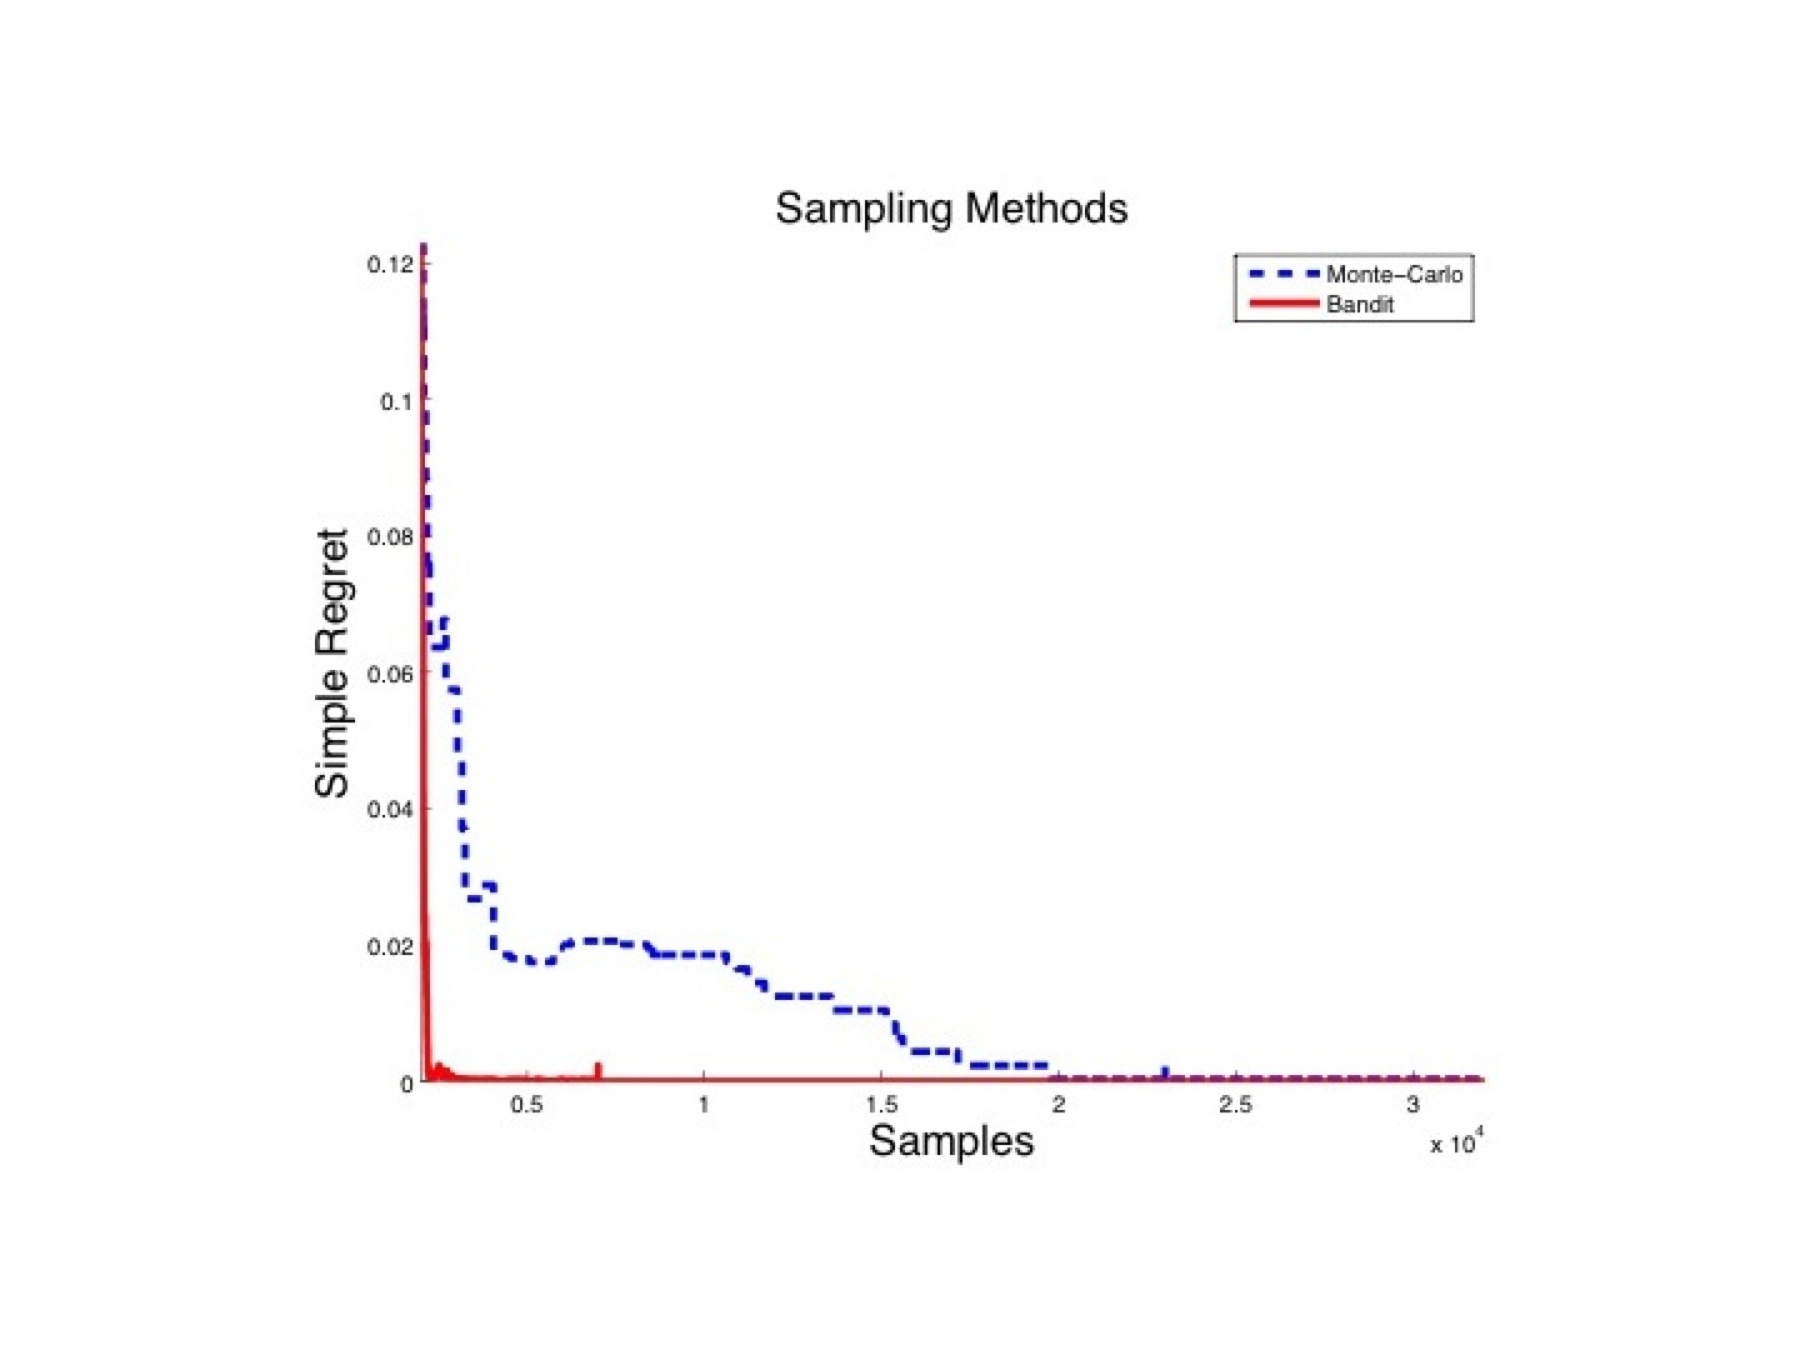
\includegraphics[width = 6cm, height = 4cm]{figures/Slide01.jpg}
%\caption{Illustration of a grasp plan $\Gamma$ composed of two lines of action, $\gamma_1(t)$ and $\gamma_2(t)$}
%\vspace*{-10pt}
%\label{fig:line_of_action}
%\end{figure}

\begin{figure}[t!]
\centering
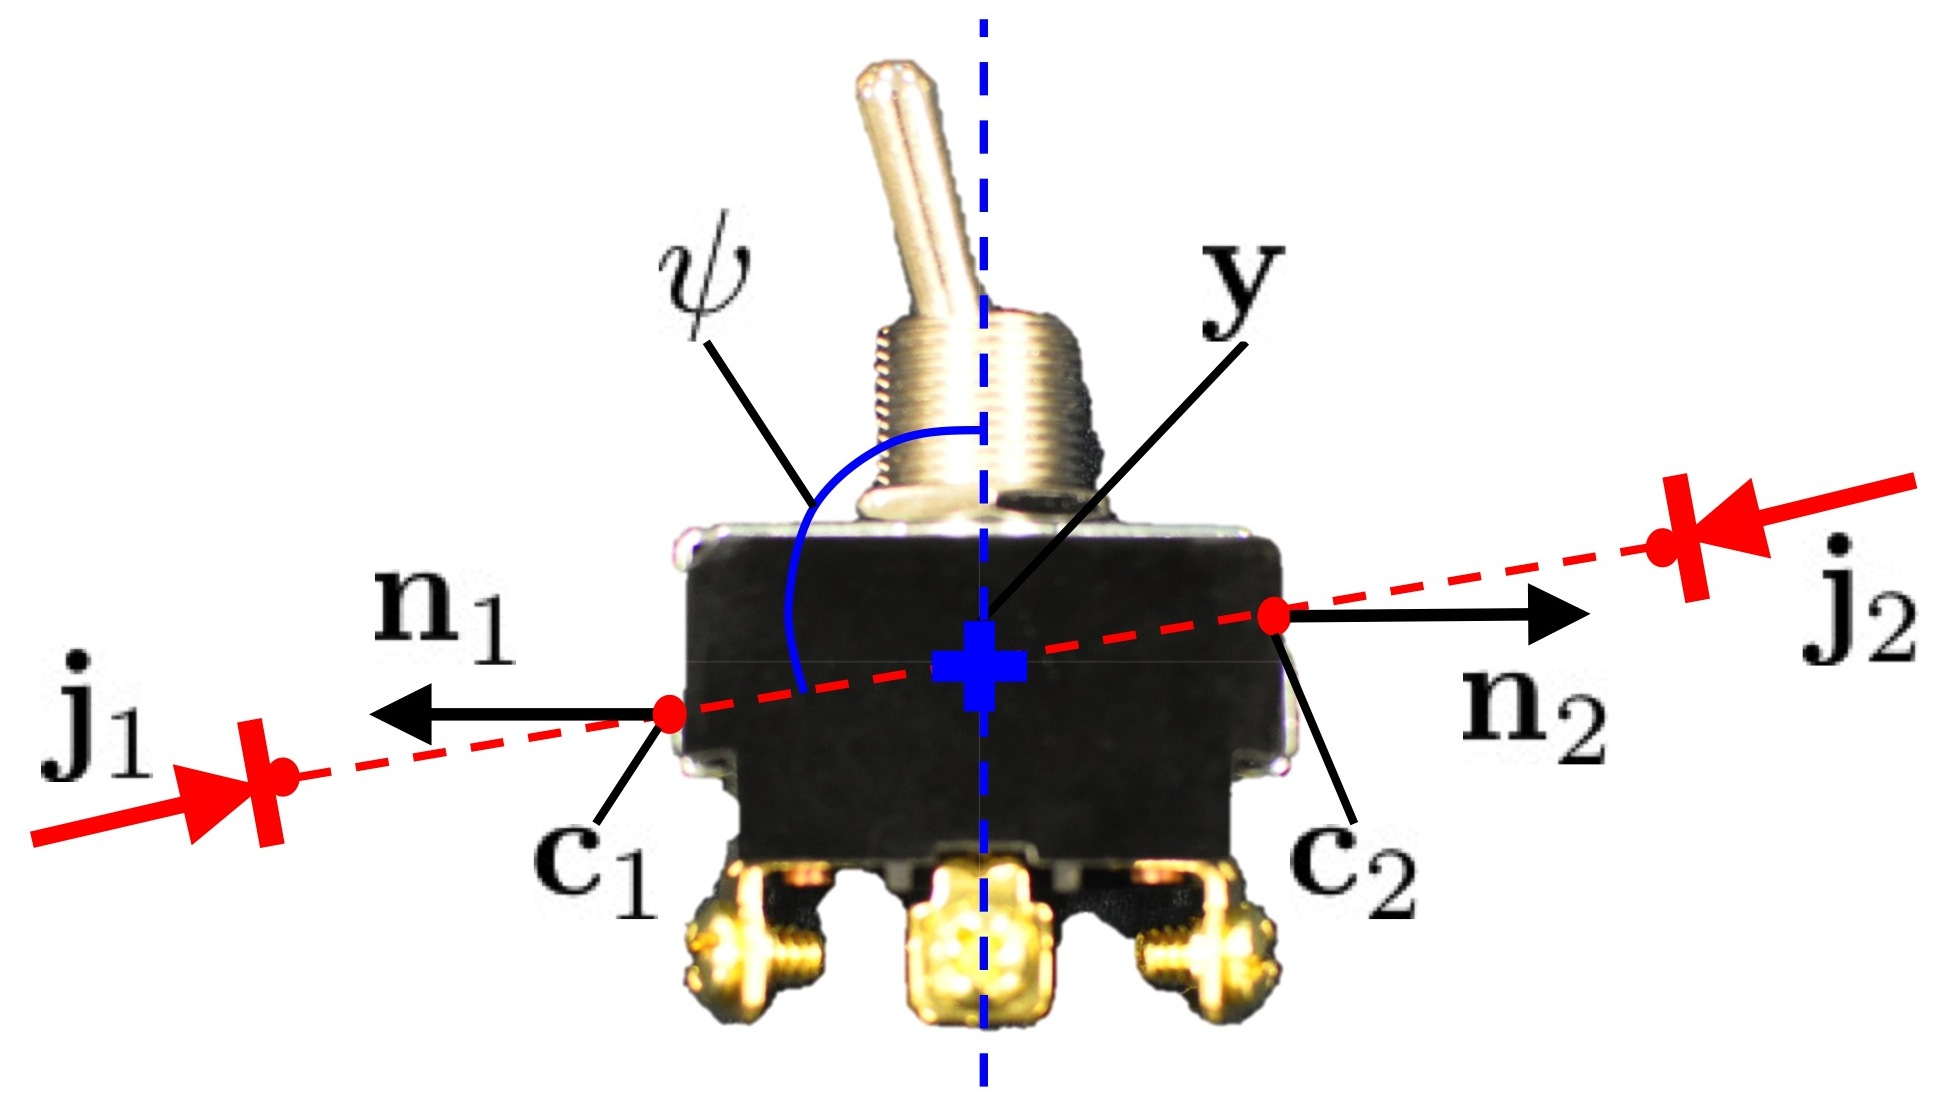
\includegraphics[width = 8.5cm, height = 5.25cm]{figures/bandit_grasp_model.jpg}
\caption{llustration of our grasping model for parallel jaw grippers on a mechanical switch. Jaw placements are illustrated by a red direction arrow and line. A grasp plan consists of 2D locations for each of the parallel-jaws $\bj_1$ and $\bj_2$. When following the grasp plan, the jaws contact the object at locations $\bc_1$ and $\bc_2$, and the object has outward pointing unit surface normals $\bn_1$ and $\bn_2$ at these locations. Together with the center of mass of the object $\bz$, these values can be used to determine the forces and torques that a grasp can apply to an object.}
\vspace*{-2ex}
\label{fig:grasp_model}
\end{figure}

\subsection{Sources of Uncertainty}
In this work we consider uncertainty in shape, pose, approach, and friction coefficient.
Fig. \ref{fig:graphical_model} illustrates a graphical model of the relationship between these sources of uncertainty.
In this section we describe each source of uncertainty and our model of the uncertainty.

\begin{figure}[ht!]
\centering
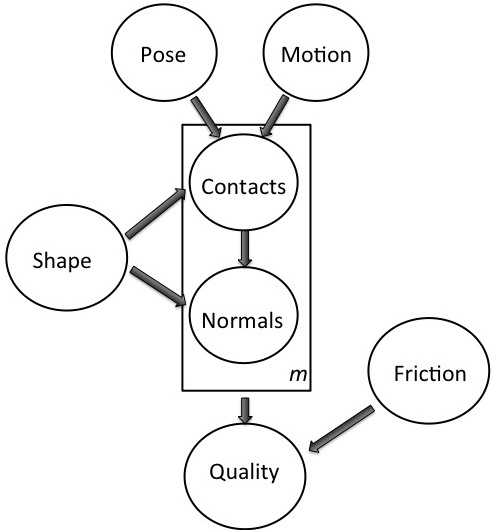
\includegraphics[width = 6cm, height = 6cm]{figures/Graphical_Model.jpg}
\caption{A graphical model that illustrates the relationship between the different types of uncertainty in an object. As illustrated uncertainty in pose, motion and shape affect the contacts and surface normals that makes up the grasp. Friction coefficient is independent of this relationship. The box around contact and normals means they are repeated nodes, in this case we have $m=2$ corresponding to the two jaws in the gripper.  }
\vspace*{-10pt}
\label{fig:graphical_model}
\end{figure}

\subsubsection{Shape Uncertainty}

Uncertainty in object shape results from sensor noise and missing sensor data, which can occur due to transparency, specularity, and occlusions~\cite{mahler2015gp}.
Following ~\cite{mahler2015gp}, we represent the distribution over possible surfaces given sensing noise using a Gaussian process implicit surface (GPIS).
A GPIS represents a distribution over signed distance functions (SDFs).
A SDF is a real-valued function $f: \mathbb{R}^d \rightarrow \mathbb{R}$ that is greater than 0 outside the object, 0 on the surface and less than 0 inside the object.
A GPIS is a Gaussian distribution over SDF values at a fixed set of query points $\mX = \{\bx_1, ... \bx_n\}, \bx_i \in \mathbb{R}^2$, $f(\bx_i) \sim \mN(\mu_{f}(\bx_i),\Sigma_{f}(\bx_i))$, where $\mu_{f}(\cdot)$ and $\Sigma_{f}(\cdot)$ are the mean and covariance functions of the GPIS~\cite{rasmussen2006}.
See Mahler et al. for details on how to estimate a mean and covariance function and sample shapes from a GPIS~\cite{mahler2015gp}.
Following Mahler et al., we set $\mX$ to a uniform $M \times M$ grid of points with square cells.
For convenience, in later sections we will refer to the GPIS parameters as $\theta = \lbrace \mu_{f}(\bx), \Sigma_{f}(\bx) \rbrace$. 


\subsubsection{Pose Uncertainty}
In 2-dimensional space, the pose of an object $T$ is defined by a rotation angle $\phi$ and two translation coordinates $\bt = (t_x, t_y)$, summarized in parameter vector $\mathbf{\xi} = (\phi, \bt)^T \in \mathbb{R}^3$:

\vspace{-2ex}
\begin{align*}
	T &= \left[  \begin{array}{ccc}
		\cos(\phi) & -\sin(\phi) & t_x \\
		\sin(\phi) & \cos(\phi) & t_y \\
		0 & 0 & 1
		\end{array} \right] .
\end{align*}

%One challenge with pose is that the pose matrix $T$ is used to apply pose perturbations to an object in practice, but uncertainty is mathematically more easily quantified in terms of the pose parameters $\xi$.
\todo{Jeff fix this}
\noindent Following Barfoot and Furgale, we assume that we are given a mean pose matrix $\bar{T} \in SE(2)$ and zero-mean Gaussian uncertainty on the pose parameters $\mathbf{\xi} \sim \mN \left( \mathbf{0}, \Sigma_{\xi} \right)$.~\cite{barfoot2014Pose}.

 
 \subsubsection{Approach Uncertainty}
In practice a robot may not be able to execute a desired grasp plan $\Gamma = \lbrace \bj_i,\bj_2\rbrace$ exactly due to errors in actuation or feedback measurements used for trajectory following~\cite{kehoe2012estimating}.
We model approach uncertainty as Gaussian uncertainty around the angle of approach and centroid of a straight line grasp plan $\Gamma$.
Formally, let $\hat{\by} = \frac{1}{2} (\bj_1 + \bj_2)$ denote the center of a planned grasp axis and $\hat{\psi}$ denote the angle that the planned axis $\bj_1 - \bj_2$ makes with the x-axis of the 2D coordinate system on our shape representation.
We model uncertainty in the approach center as $\by \sim \mN(\hat{\by}, \Sigma_y)$ and uncertainty in the approach angle as $\psi \sim \mN(\hat{\psi}, \sigma_{\psi}^2)$.
For shorthand in the remainder of this paper we will refer to the uncertain approach parameters as $\rho = \{\by, \psi \}$.
In practice $\Sigma_{y}^2$ and $\sigma_{\psi}^2$ can be set from repeatability measurements for a robot~\cite{mooring1986determination}.

 \subsubsection{Friction Uncertainty}
As shown in \cite{zheng2005}, uncertainty in friction coefficient can cause grasp quality to significantly vary.
However, friction coefficients may be uncertain due to factors such as material between a gripper and an object (e.g. dust, water, moisture), variations in the gripper material due to manufacturing tolerances, or misclassification of the object surface to be grasped.
We model uncertainty in friction coefficient as Gaussian noise, $\mu \sim \mN(\hat{\mu},\sigma_{\mu}^2)$.


\vspace{-2ex}
 
\subsection{Grasp Quality}\label{sec:grasp_sample}
We measure the quality of grasp using the probability of force closure~\cite{weisz2012pose, kim2012physically, kehoe2012estimating, kehoe2012toward} given a grasp plan $\Gamma$. Force closure is a binary-valued quantity $F$ that is 1 if the grasp can resist wrenches in arbitrary directions and 0 otherwise.
Let $\mW \in \mathbb{R}^3$ denote the contact wrenches derived from contact locations $\bc_1,\bc_2$, normals $\bn_1,\bn_2$, friction coefficient $\mu$, and center of mass $\bz$ for a given grasp and shape.
If the origin lies within the convex hull of $\mW$, then the grasp is in force closure~\cite{li1988task}.
We rank grasps using the probability of force closure given uncertainty in shape, pose, robot approach, and friction coefficient~\cite{christopoulos2007handling, kehoe2012toward}:

\vspace{-2ex}
\begin{align*}
	P_F(\Gamma) &= P \left(F = 1 | \Gamma, \theta, \xi, \rho, \mu \right).
\end{align*}

 
To estimate $P_F(\Gamma)$, we generate samples from each of the distributions in sequence using the relationships defined by the graphical model in Fig. \ref{fig:graphical_model}.
After sampling a shape, pose, approach direction, and friction coefficient, we compute the contact locations $\bc_i$ and the surface normals $\bn_i$ using Bayes rule:
 
 \vspace{-2ex}
 \begin{align*}
 &p(\textbf{n}_i,\textbf{c}_i |\gamma_i(t),\theta,\xi,\rho)=\\
 &p(\textbf{n}_i|\textbf{c}_i,\theta)p(\textbf{c}_i|\gamma_i(t),\theta,\rho,\xi)
 \end{align*}

 
Mahler et al.describe how to draw shape samples from a GPIS model ~\cite{mahler2015gp}.
We next sample from $p(\xi)$ and $p(\rho)$ to compute $p(\textbf{c}_i|\gamma_i(t),\theta,\rho,\xi)$ via ray tracing along the grasp axis defined by $j_1$ and $j_2$~\cite{newcombe2011kinectfusion}.
Then $p(\textbf{n}_i|\textbf{c}_i,\theta)$ corresponds to the normal vector at the sampled contact point.We use these quantities to compute the forces and torques that can be applied to form the contact wrench set $\mW$ and evaluate the force closure condition \cite{li1988task}.



\subsection{Objective}
\seclabel{objective}

Given the sources of uncertainty and their relationships as described above, the grasp planning objective is to find the grasp that maximizes the probability of force closure from a set of candidate grasps $\mG = \{\Gamma_1, ..., \Gamma_K\}$:

\vspace{-2ex}
\begin{align}
\Gamma^* &= \underset{\Gamma_k \in \mG}{\text{argmax }} P_F\left( \Gamma_k\right) \label{eq:old_problem_def}
\end{align}

% Since we only can approximate the probability of force closure, with samples drawn from the distribution $P_F(\Gamma)$ our objective is rewritten as: 

% \vspace{-2ex}
% \begin{align}
% \Gamma^* &\approx \underset{\Gamma \in \mG}{\text{argmax }} P\left( F = 1 | \Gamma, \theta, \xi, \rho, \mu \right) \label{eq:problem_def}
% \end{align}

One method to approximately solve Equation~\ref{eq:old_problem_def} is to exhaustively evaluate $P_F(\Gamma_k)$ for all grasp plans in $\mG$ using Monte-Carlo integration and then sort the plans by this quality metric, we refer to this as a brute force approach. 
This method has been evaluated for shape uncertainty~\cite{christopoulos2007handling, kehoe2012estimating} and pose uncertainty~\cite{weisz2012pose} but may require many samples for each of a large set of candidates to converge to the true value.
More recent work has considered adaptive sampling to discard grasp plans that are not likely to be optimal without fully evaluating their quality~\cite{kehoe2012toward}.
\todo{improve this tomorrow }

To try and reduce the number of samples needed, we instead maximize the sum of $P_F$ values for each sampled grasp plan $\Gamma_{k,t}$ at time $t$ up to a given time $T_s$:
\begin{align}
    \underset{\Gamma_{k,} \in \mG}{\text{argmax }} \sum \limits_{t=1}^
    {T_s} P_F \left( \Gamma_{k,t}\right)  \label{eq:problem_def}
\end{align}
\noindent This tries to perform as well as Equation~\ref{eq:old_problem_def} in as few samples as possible~\cite{srinivas2009gaussian}.We then formulate  problem as a MAB model and compare two different Bayesian MAB algorithms, Thompson Sampling and Gittins Indices.

\section{Grasp Planning as a Multi-Armed Bandit}
We frame the grasp selection problem of \secref{objective} as a multi-armed bandit problem.
Each arm corresponds to a different grasp plan, $\Gamma_k$, and pulling an arm corresponds to sampling from the graphical model in Fig. \ref{fig:graphical_model} and evaluating the force closure condition.Since force closure is a binary value, each grasp plan $\Gamma_k$ has a Bernoulli reward distribution with probability of force closure, $P_F(\Gamma_k)$.
In a MAB, we want to try and minimize cumulative regret which is an equivalent objective to the objective of Equation~\ref{eq:problem_def}.

One can think of the proposed algorithm as an anytime algorithm. It can be stopped at anytime during its computation and return the current estimate of the best grasp or wait until a $95\%$ confidence interval is smaller than some threshold $\epsilon$. Using the quantile function of the beta distribution, $B$, we can measure the $95\%$ confidence interval as: 

\vspace{-2ex}
\begin{align}\label{eq:confidence}
B(0.05,\alpha_{k,n},\beta_{k,n}) \leq P_F(\Gamma_k)) \leq B(0.95,\alpha_{k,n},\beta_{k,n})
\end{align}

To summarize the algorithm terminates when the following OR condition is meet 

\vspace{-2ex}
\begin{align}\label{eq:stopping_condition}
\lbrace t \geq T_s \: \mbox{OR} \: |B(0.05,\alpha_{k,n},\beta_{k,n}) -  B(0.95,\alpha_{k,n},\beta_{k,n})| \leq \epsilon \rbrace
\end{align}
where the $k$ grasp plan refers to the one that is currently being returned. 
 .
\section{Simulation Experiments}
We used the Brown Vision Lab 2D dataset \cite{brown}, a database of object ,  the same as in \cite{christopoulos2007handling}.Examples of the objects can be seen in \ref{fig:shape_samples}.  We down sampled the image by a factor of 2 to create a 40 x 40 occupancy map, which holds 1 if the point cloud was observed and 0 if it was not observed, and a measurement noise map, which holds the variance 0-mean noise added to the SDF values. We estimate the GPIS using the same method proposed in \cite{mahler2015gp}. For illustrative purposes of noise, the noise of the motion, position and friction coefficient was set to the following variances $\sigma_{mot} = 0.2$ rads, $\sigma_{mu} = 0.4$, $\sigma_{rot} = 0.3$ rads and $\sigma_{trans} = 3$ grid cells.
We performed experiments for the case of two hard contacts in 2-D. We drew random grasp plans $\Gamma$ by sampling the angle of grasp axis around a circle with radius $\sqrt{2} M$, where $M$ is the dimension of the workspace, and then sampling the circle's origin. 





\subsection{Multi-Armed Bandit Experiments}
For our experiments we look at selecting the best grasp out of a size of $|G| = 1000$. We initialize all algorithms by sampling each grasp 1 time. We draw samples from our graphical model using the technique described in Sec.  \ref{sec:grasp_sample}. In Fig. \ref{fig:grasp_quality}, we plotted the probability of force closure, $P_F$, of the grasp chosen vs. stopping time $T_s$ averaged over 100 randomly selected shapes in the Brown Vision Lab 2D dataset and compare the four different methods (Thompson, Gittins, Iterative Pruning \cite{kehoe2012toward} and uniform allocation). Uniform allocation selects a grasp at random from the set to sample next, thus does not use any prior information. Iterative Pruning prunes grasps every 1000 iterations based on lowest sample mean and removes 10$\%$ of the current grasp set.  We set the discount factor $\gamma =0.98$ for Gittins because that was the highest we could compute the indices for, since it scales exponentially in computation. 

\todo{This might still be vague} As illustrated in Fig. \ref{fig:grasp_quality}, Gittins and Thompson select a grasp at stopping time $T_s$ that on average has a higher probability of force closure than uniform allocation and Iterative Pruning . For illustrative purposes of an anytime algorithm,  we select a stopping time $T_s=1000$, which is only 10 samples per grasp on average, and for each method visualize the grasp selected in Fig. \ref{fig:shape_samples}. 

 The MAB algorithm can also be terminated not at a fix stopping time $T_s$, but at the time when the $95\%$ confidence interval, Eq. \ref{eq:confidence}, around the returned grasp is below a set threshold $\epsilon$. We plot the confidence intervals around the return grasp vs. the number of samples drawn in Fig. \ref{fig:confidence} for Thompson Sampling, Iterative Pruning\cite{kehoe2012toward} and uniform allocation. \todo{Still thinking of a way to quantify this} As illustrated, the confidence interval for Thompson sampling converges at a faster rate than the other two methods. 

 In our experiments the MAB methods honed in their sampling efforts on promising grasps, for the top 10$\%$ of grasps Thompson Sampling allocates 29$\%$ of the total number of samples and Gittins allocates 23$\%$ of total samples. Uniform allocation and Iterative Pruning allocate $1\%$  and $6\%$ of total samples, respectively. In Fig. \ref{fig:pulls_per_grasp}, we plot samples per grasp quality. Gittins and Thompson appear to allocate  more samples to grasps of higher estimated probability of force closure in contrast to uniform allocation and Iterative Pruning. The focused sampling on higher quality grasp can explain the ability to find grasps with a higher probability of force closure  faster and have a smaller confidence interval on the returned quantity. 
 
 


\begin{figure}[t!]
\centering
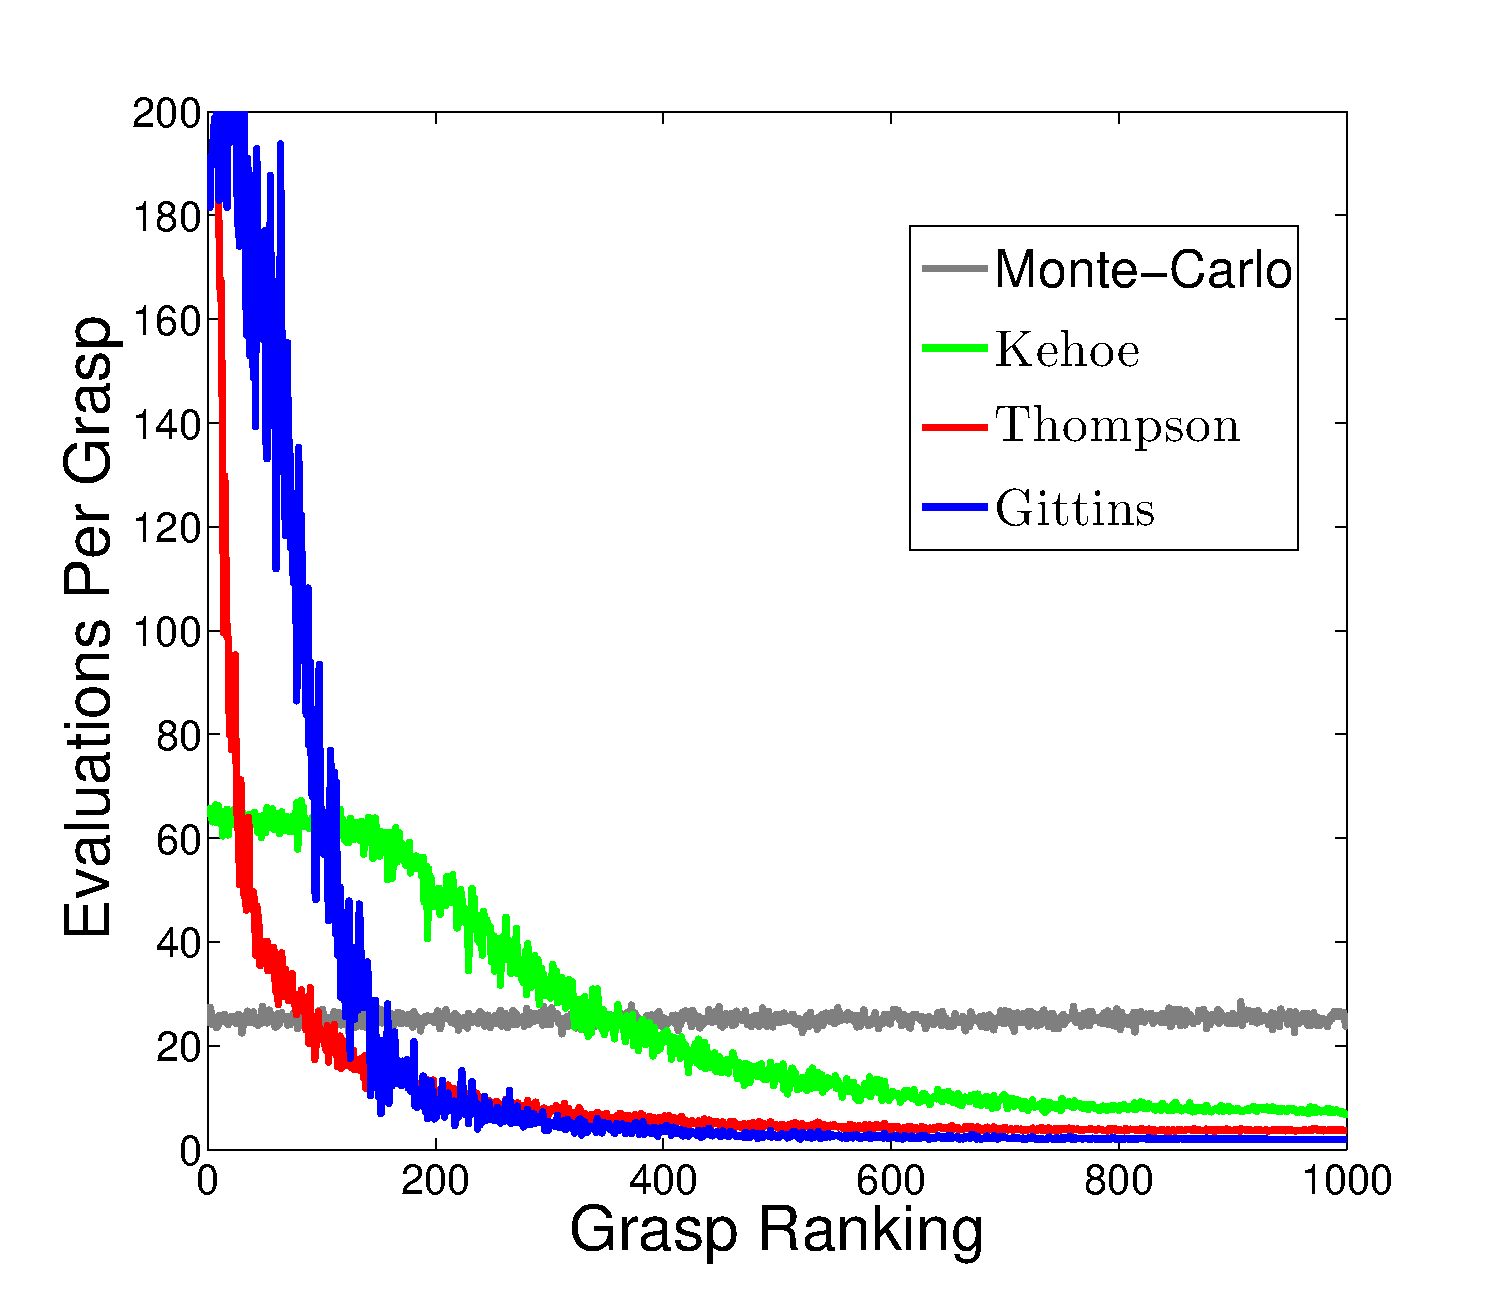
\includegraphics[scale=0.25]{matlab_figures/pulls_per_grasp.eps}
\caption{ \footnotesize Comparison of sample per grasp for the four sequential decision methods (Thompson, Gittins, uniform allocation and Iterative Pruning). Graph is averaged over 100 objects from the Brown Silhouette Dataset \cite{brown} with a set $|G|=1000$ for each object. The best grasps are ranked 1 and worst are 1000. As illustrated the MAB algorithms intelligently allocate samples towards high quality grasps based on past observations, where Monte-Carlo Integration takes a uniform approach to allocation. }

\vspace*{-10pt}
\label{fig:pulls_per_grasp}
\end{figure}

\begin{figure}[t!]
\centering
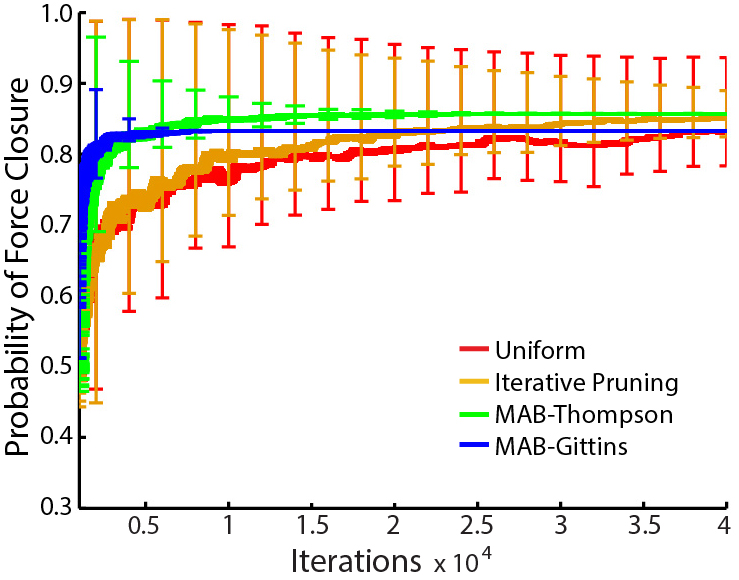
\includegraphics[scale=0.25]{matlab_figures/confidence_bounds.eps}
\caption{ \footnotesize \todo{We might want to condense Fig 6 and Fig. 4. The confidence intervals clutter the plot though} The probability of Force Closure of the grasp returned vs the number of samples required with a $95\%$ confidence interval around the return value for Thompson Sampling, Iterative Pruning and uniform allocation. Graph is averaged over 100 objects from the Brown Silhouette Dataset \cite{brown} with a set $|G|=1000$ for each object. The sharper decrease in confidence interval corresponds to more samples being allocated for the return grasp. }

\vspace*{-10pt}
\label{fig:confidence}
\end{figure}


\begin{figure*}%
\label{fig:shape_examples}
    \centering
    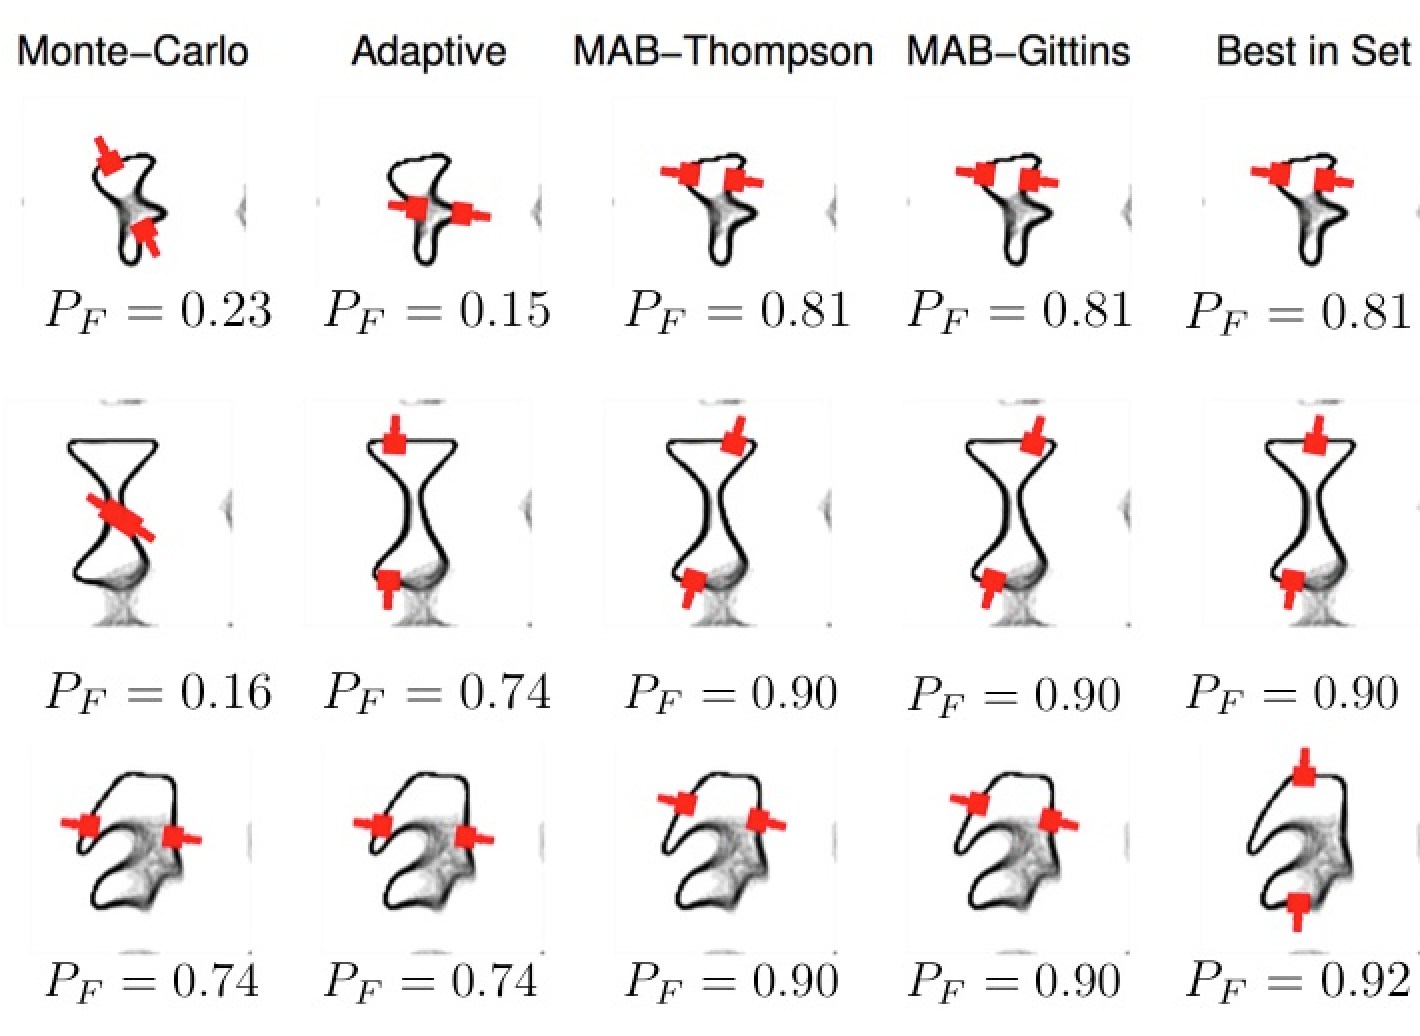
\includegraphics[width=16.5cm]{figures/shapes.png}%
  
    \caption{\todo{Need to change this figure, wondering what should be conveyed here}Three objects shown from the Brown Visual Lab Dataset with induced shape uncertainty and visualized with the GPIS-Blur method \cite{mahler2015gp}. The four methods (uniform allocation, Iterative Pruning, Thompson and Gittins) were all run until a stopping time of $10,000$ evaluations with a randomly selected grasp set of $|G|=1000$. We also show the grasp returned by the brute force approach of exhaustively sampling every grasp in the set.  The grasps and the quality each one found is shown above.  In the two out of three cases, Thompson sampling is able to find the best grasp in the set at the stopping interval of $10,000$, however at the last shape there is a difference of $2\%$ grasp quality.   }%
    \label{fig:shape_samples}%
\end{figure*}


\subsection{Sensitivity Analysis }\label{sec:sensitivity}
\todo{need to redo with larger number of shapes}
We now will show how well  Thompson Sampling perform under a variation in noise from friction coefficient uncertainty, shape uncertainty, rotational pose and translation pose and use that to set the parameters for future experiments . The experiments are performed with the same setup as before but now we increase the variance parameters across a set range for each parameter to simulate low, medium and high levels of noise. All experiments were averaged across 10 shapes randomly selected with from the Brown dataset with $|G| = 1000$, or 1000 grasp plans $\Gamma$. 

For friction coefficient we varied $\sigma_{\mu}$ across the following values $\sigma_{\mu} = \lbrace 0.05, 0.2, 0.4 \rbrace$. As illustrated in Table 1, the performance of the bandit algorithm remains largely unchanged, with typical convergence to zero in simple regret less than 2000 evaluations.

For rotational uncertainty in pose, we varied $\sigma_{rot}$ over the set of $\lbrace 0.03, 0.12,0.24\rbrace$ radians. As illustrated in Table 1, the performance of the bandit algorithms is effected by the change in rotation, increase in variance to $0.24$ radians or $13^{\circ}$  causes the convergence in simple regret to not be reached until around 4432 samples or an average of 5.5 samples per grasp. 

For translational uncertainty in pose, we varied $\sigma_{trans}$ in the range of $\lbrace 3,12, 24 \rbrace$ units (on a 40 x 40 unit workspace). As you can see in Table 1, the performance of the bandit algorithms is effected by the change in rotation, increase noise of $\sigma_{trans} = 24$ causes the convergence to not be reached until 8763 evaluations for Thompson Sampling. 



\subsection{Worst Case}
The MAB algorithms use the observations of samples drawn to decide which grasp to sample next from. To show worst case performance under such a model, we sorted the quality of all 1000 grasps offline and arranged the order of samples, so that the top 500 grasps have samples drawn in the order of worst to best and the bottom 500 grasps have samples drawn in order of best to worst. The intent here is to provide misleading observations to the bandit algorithms. We demonstrate in Fig. \ref{fig:worst_case} a case where the observations are misleading. 

As illustrated in Fig. \ref{fig:worst_case}, all the methods are affected by worst case performance. It would appear that when the observations are misleading the best thing to do is simply uniform allocation of grasp samples. One interesting aspect that is illustrated is that Thompson sampling is able to make improvement while the other two methods are stuck in local optimal. This is because Thompson sampling is guaranteed to find the best grasp in the limit of infinite iterations \cite{agrawal2011analysis}.



\begin{figure}[t!]
\centering
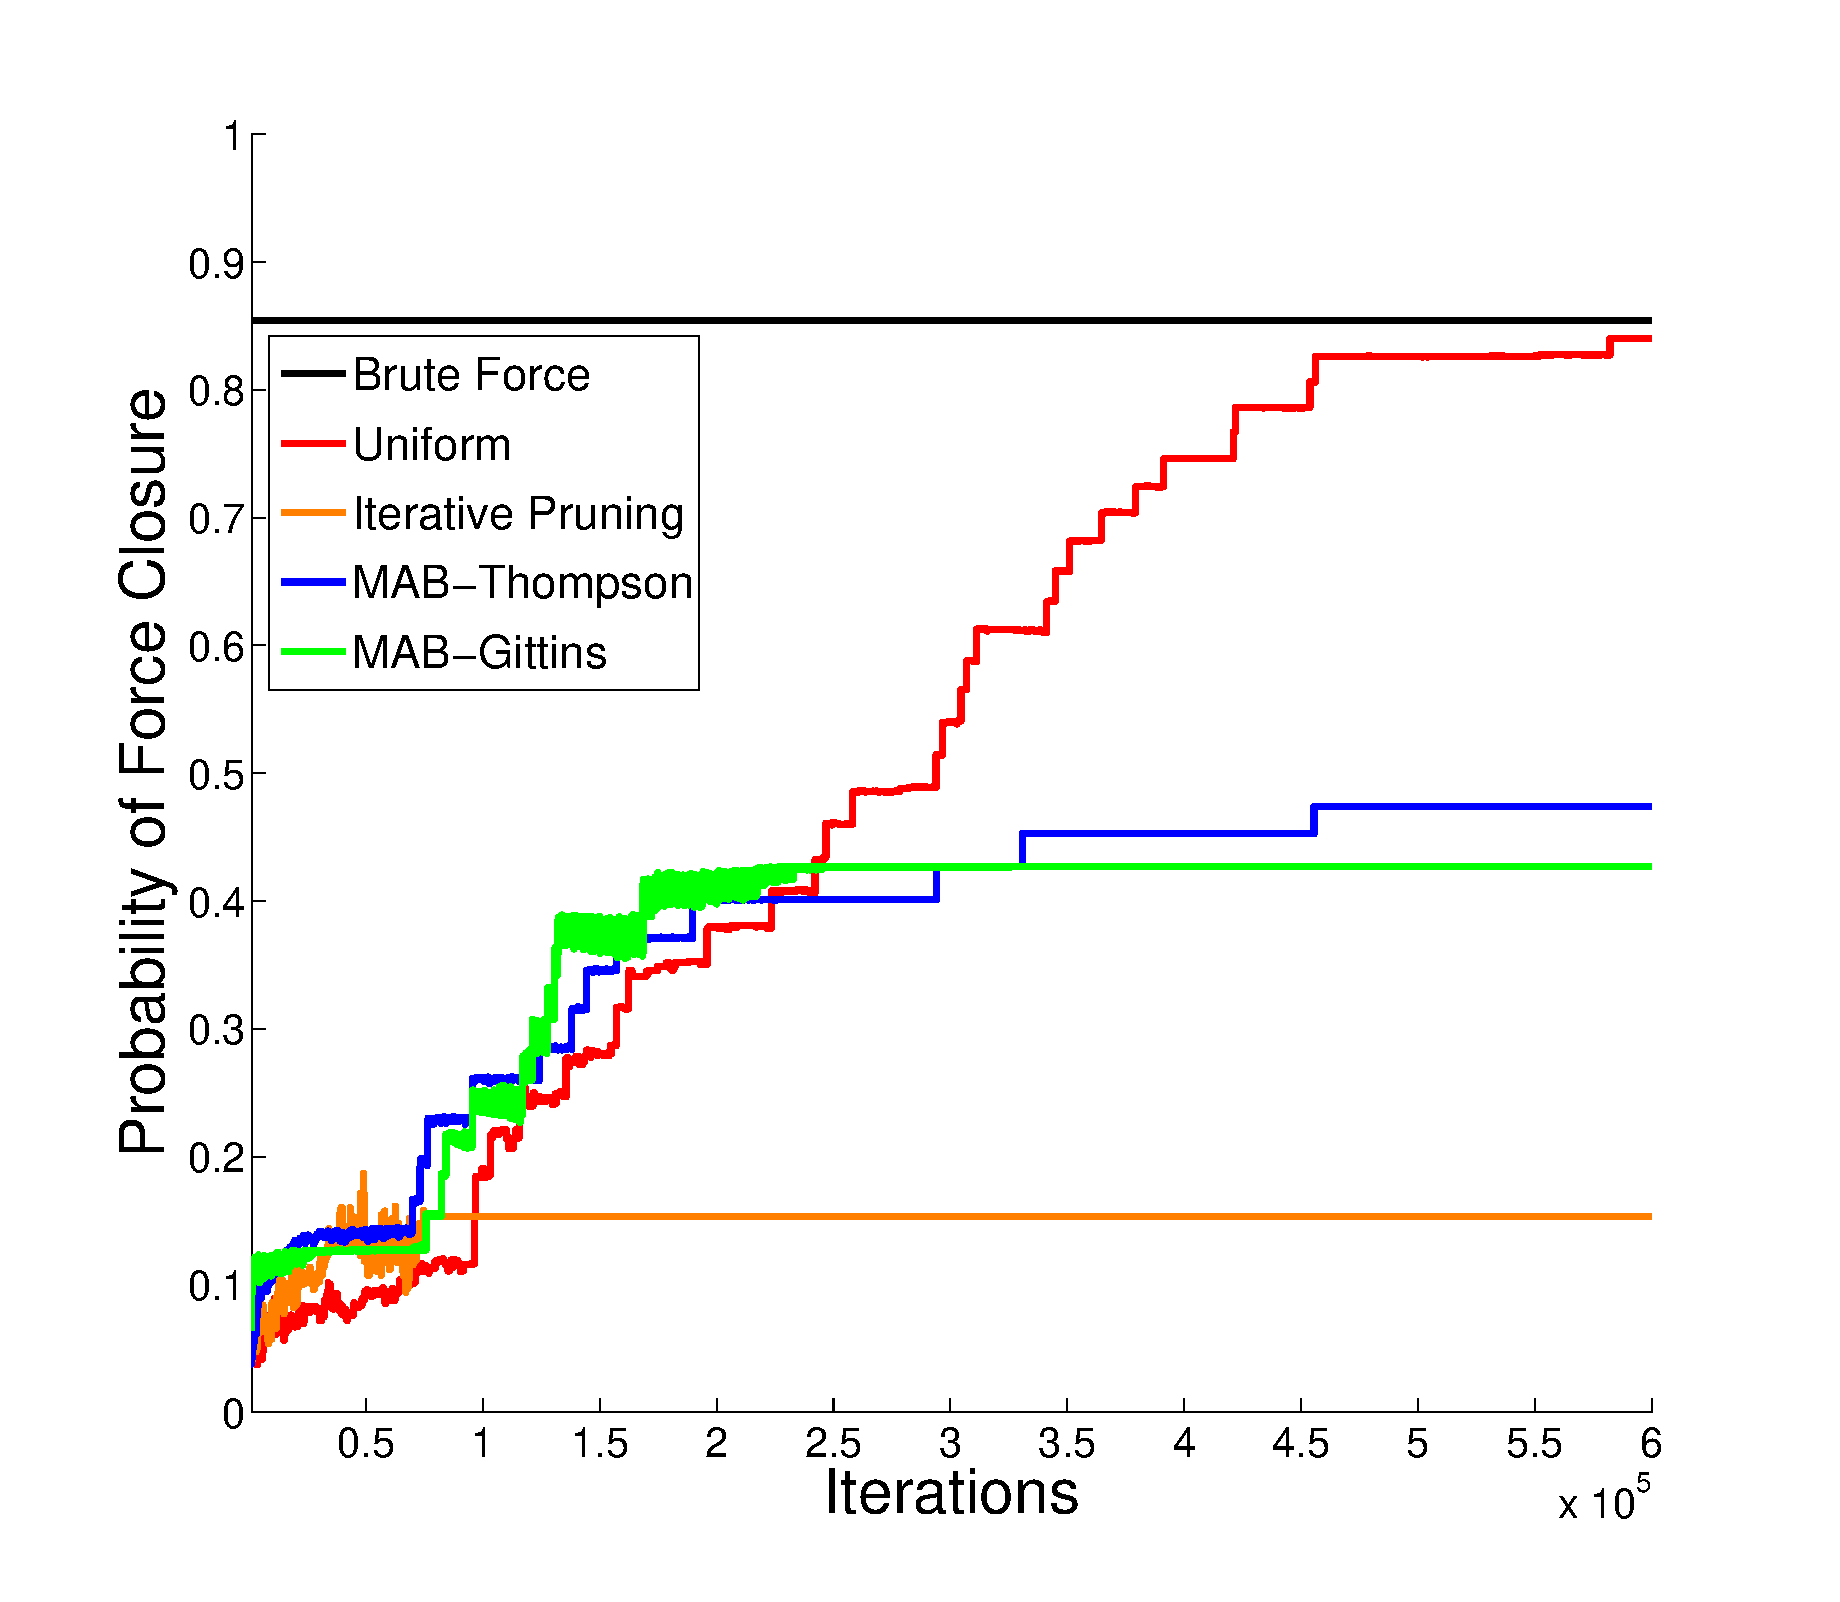
\includegraphics[scale=0.25]{matlab_figures/worst_case.eps}
\caption{ \footnotesize Comparison of the current average probability of force closure vs. the stopping time $T_s$ for the pathological case where the samples are sorted to be misleading. The graph is averaged over 100 objects randomly drawn from the Brown Vision 2D Lab Dataset \cite{brown} with a set $|G|=1000$ for each object.  We demonstrate this for Thompson, Gittins, uniform allocation and Iterative Pruning \cite{kehoe2012estimating}. We also demonstrate what the average highest probability of force closure is when the brute force approach of exhaustively sampling each candidate grasp is used. Empirically, it appears that when samples are misleading the best policy is uniform allocation. However, it also illustrated that Thompson sampling can recover from this situation where Gittins and Kehoe et al.  are not able to and get stuck in local solutions. }
\vspace*{-10pt}
\label{fig:worst_case}
\end{figure}


\begin{table*}[t]
\centering
\begin{tabular}{ |p{4.5cm}||p{2cm}|p{2.5cm}|p{2cm}|  }
 \hline
 \multicolumn{4}{|c|}{Sensitivity Analysis for Convergence to Best Grasp for Thompson Sampling} \\
 \hline
Uncertainty Type & Low Uncertainty ($\#$ of Iterations) & Medium Uncertainty ($\#$ Iterations) & High Uncertainty ($\#$ of Iterations)\\
 \hline
Translation Variance in Pose, $\sigma_{trans}$ & 1210    & 2207 &  8763\\
Friction Coefficient Variance, $\sigma_{fric}$ &  1985  & 1456   & 1876\\
Rotational Variance in Pose, $\sigma_{rot}$ & 4230 & 4431 &  4432\\
 \hline
\end{tabular}
   \caption { \footnotesize  Sensitivity Analysis for convergence to estimated best grasp for Thompson Sampling under rotational variance $\sigma_{rot} = \lbrace 0.03,0.12, 0.24 \rbrace$ radians,  translation uncertainty $\sigma_{trans} = \lbrace 3, 12, 24 \rbrace$ units  friction coefficient uncertainty $\sigma_{fric} = \lbrace 0.05,0.2, 0.4 \rbrace$  from left to right on a 40 x 40 unit workspace averaged over 10 objects from the Brown Vision Lab Data set. The sensitivity analysis shows that large variance in translational uncertainty in pose can increase the amount of iterations needed for the bandit algorithm to converge to the highest quality grasp in the set. 
   }
		\tablabel{opt-p-comparison}
\vspace*{-20pt}
\end{table*}


\section{Discussion and Future Work } 

Assessing grasp quality under  uncertainty can be computationally expensive as it often requires repeated evaluations of the grasp metric over many random samples.
In this work, we proposed a multi-armed bandit approach to efficiently identify high-quality grasps under uncertainty in shape, pose, friction coefficient and approach. 
A key insight from our work is that exhaustively sampling each grasp is inefficient, and we found that a MAB approach gives priority to promising grasps and can reduce computational time. Initial results have shown our MAB approach to outperform the methods of prior work, uniform allocation and Iterative Pruning  \cite{kehoe2012toward}\cite{kehoe2012estimating} in terms of finding a higher quality grasp faster. 
 However, as shown in Fig. \ref{fig:worst_case} there can exists pathological cases that can mislead bandit algorithms to focus samples on the wrong grasps. Fortunately, though these cases occur with a small very probability, however it is important for a practitioner to be aware of them. 

In future work, we plan to scale our method to 3D objects. However, this could substantially increase the number of candidate grasp plans. To handle a much larger amount of arms, it becomes neccesary to have some measure of correlation between them. If two grasps are similar with respect to some metric, then their measure of probability of force closure should be correlated. Appropriate features that represent an grasp under uncertainty  and the metric itself are still open questions though and will be an ongoing project for future work. 
\bibliographystyle{IEEEtranS}
\bibliography{references}



\end{document}
